\chapter{Introduction}
Artificial intelligence (AI) is widely used in board games. It is an efficient solution, but the task becomes very complicated when uncertainty comes into play. It creates a lot of possible options for the game's development, and it becomes challenging to predict different possibilities. One of such games is Backgammon.

Nowadays, we can utilize AI to play games with uncertainty and understand them better. Computers can simulate thousands of games relatively quickly, which helps us discover new strategies and decisions that improve gameplay. This thesis is about teaching a computer to play Backgammon intelligently using methods that handle uncertainty, similar to how human players adapt to changing dice rolls.
The topic is important because understanding how to improve the computer's game decisions helps us learn about decision-making under uncertainty.
Even now, when AI has improved significantly, easily surpassing human champions in many games, these games are not solved, and we are constantly looking for more optimal solutions. There is always room to grow and become more effective.

The main goal of this thesis is to implement a specific AI algorithm known as ExpectiMiniMax to play Backgammon. By simulating many AI versus AI matches, the thesis examines which factors genuinely impact the quality of the game and uses this knowledge to improve how the computer evaluates different game positions.

 Chapter \ref{Backgammon} covers the basics of Backgammon, its rules, and how it is traditionally played. Chapter \ref{AI algorithms} explains AI algorithms and provides background on how computers make decisions. Chapter \ref{Implementation} describes the implementation of the Backgammon game itself in C\# language and the ExpectiMiniMax algorithm. Chapter \ref{Optimizations} is dedicated to how to optimize this implementation for better performance. Chapter \ref{Evaluation} examines the factors impacting game outcomes and how to improve the evaluation of game states. In this chapter, the impact of these factors on the game was experimentally determined.

\chapter{Backgammon}\label{Backgammon}
Backgammon is a two-player game where each participant moves their checkers according to the outcomes of dice rolls. It is one of the oldest known board games, which combines both strategy and probability. 
This section recaps the game's rules, which form the basis for implementing the game's code and the ExpectiMiniMax algorithm. Details about this algorithm will be provided in the following chapters.

\section*{Rules of Backgammon}
The game rules and terminology were adapted from the Backgammon Galore website \cite{rules}.

\begin{itemize}
    \item The objective of \textbf{Backgammon} is for a player to move all of their \textbf{checkers} into their \textbf{home board} and then \textbf{bear them off}. The first player to remove all of their checkers from the board wins the game.
    
    \item The Backgammon board consists of \textbf{24 points}. Each player has a \textbf{home board} and an \textbf{outer board}, separated by a central area called the \textbf{bar}. Each player moves in opposite directions: one clockwise, the other counterclockwise.
    
    \item Each player begins with \textbf{15 checkers} placed on specific points. The standard layout includes:
    \begin{itemize}
        \item Two checkers on the \textbf{24-point}
        \item Five on the \textbf{13-point}
        \item Three on the \textbf{8-point}
        \item Five on the \textbf{6-point}
    \end{itemize}
    This fixed setup defines the \textbf{initial game state} (Figure \ref{fig:backgammon_setup}).
    
    \item At the start of the game, each player rolls one die. The player with the higher value moves first. If players get the same die value, they re-roll again until there is a winner. In later turns, players roll \textbf{two six-sided dice} and move checkers based on the rolled values. A checker may move to:
    \begin{itemize}
        \item An unoccupied point
        \item A point occupied by the player's checkers
        \item A point with a single opposing checker (a \textbf{blot})
    \end{itemize}
    
    \item A point with \textbf{two or more opposing checkers} is \textbf{blocked} and cannot be moved to. Players must choose valid destinations and \textbf{cannot pass} unless no legal moves are available.

    \item Each die represents a separate move. A player may:
    \begin{itemize}
        \item Move \textbf{one checker} using both values
        \item Move \textbf{two checkers} separately
    \end{itemize}
    The player must use as many dice values as possible and cannot skip the turn unless there are no legal moves.
    
    If a \textbf{double} is rolled (e.g., 5--5), the player must make a move 4 times. If a player moves a single checker multiple times using both dice values, each move must be legal on its own, and the checker must land on an open or valid point at each intermediate step; blocked points cannot be passed through.
    
    \item Landing on a point with a \textbf{single opposing checker} \textbf{hits} it and sends it to the \textbf{bar}. A checker on the bar must be \textbf{re-entered} into the opponent's \textbf{home board}. Re-entry requires an \textbf{open point} matching the value of one of the dice.
    
    \item Once all checkers are in the player's home board, they may begin \textbf{bearing off}. A die roll must match the distance from a checker to the edge (point 1 for white or point 24 for black). If an exact match isn't possible, the player may bear off the \textbf{furthest checker within reach}.
    
    \item If no legal move is possible, the player must \textbf{pass his turn}. This can happen if:
    \begin{itemize}
        \item All destination points are \textbf{blocked}
        \item A checker is on the \textbf{bar} with no valid entry point
    \end{itemize}
    
\end{itemize}

\begin{figure}[H]
    \centering
    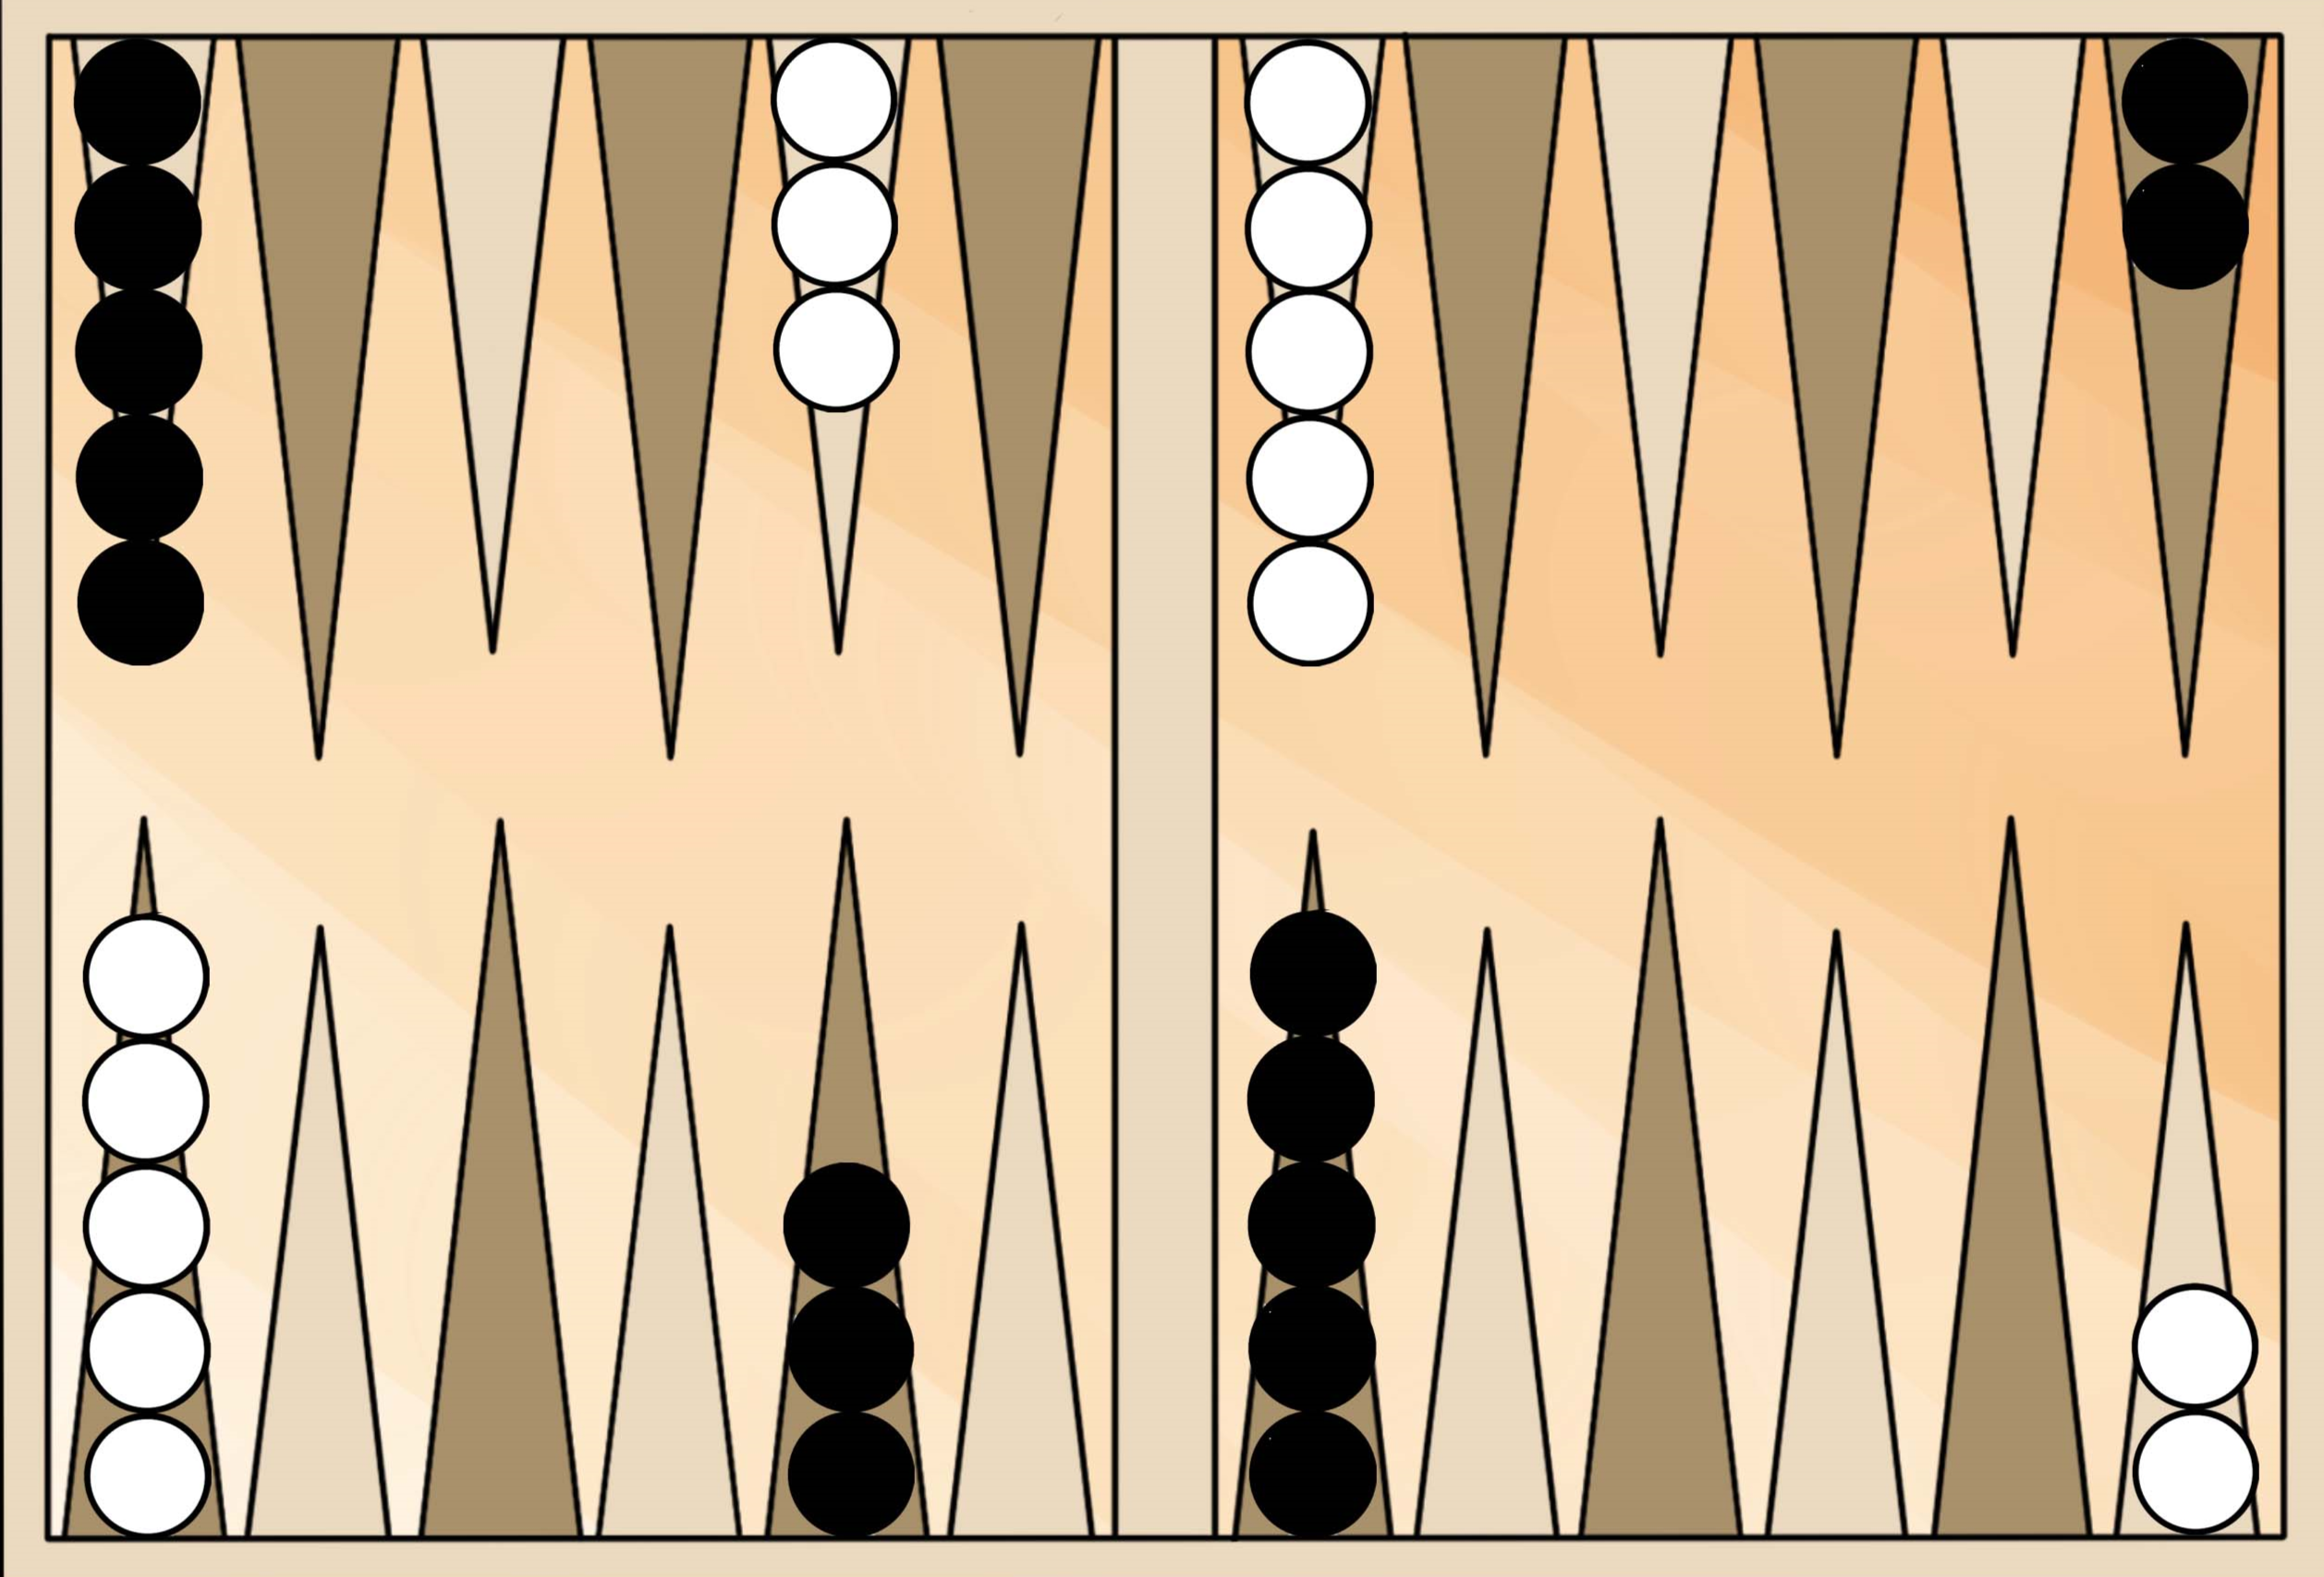
\includegraphics[width=0.8\linewidth]{obrazky-figures/Backgammon_board.png}
    \caption{Initial setup}
    \label{fig:backgammon_setup}
\end{figure}


\chapter{AI algorithms}\label{AI algorithms}
This chapter will focus on describing the usage of AI in adversarial search problems known as games. The usage is wide, involving different approaches to making a multi-agent environment. Their selection mainly depends on the game's complexity, randomness, and level of available information.
\section{Algorithms for board games}

\begin{itemize} \item \textbf{Search-based Decision-Making Algorithms} simulate rational thinking by exploring possible future game states.
Such methods as MiniMax and ExpectiMiniMax are widely used in chess and Backgammon, respectively.

\item \textbf{Reinforcement Learning (RL)} enables an AI agent to learn strategies through trial and error, receiving rewards for successful actions. TD-Gammon is a perfect example of the usage of reinforcement learning \cite{Temporal_Difference}.

\item \textbf{Monte Carlo Methods} use random simulations (rollouts) to evaluate moves and estimate outcomes. For example, Monte Carlo Tree Search (MCTS) has been used to develop AlphaGo \cite{brunner2019mastering}. Combined with neural networks, this method helped an AI defeat a human player in the game of Go for the first time in 2015 and then defeat a Go champion in 2017.

\item \textbf{Neural Networks and Deep Learning} are widely used techniques. They allow AI to learn patterns and evaluation functions directly from game data. For example, AlphaZero and MuZero combined deep neural networks with MCTS to play chess, shogi, and Go \cite{AlphaMuZero}.

\item \textbf{Evolutionary Algorithms} are inspired by natural evolution, so these methods evolve strategies or evaluation functions over generations. Such genetic algorithms have been used to train AI in Othello \cite{Lai2006ApplyingGA}.

\item \textbf{Case-Based or Imitation Learning} involves observing and mimicking expert moves from previous games. An example is training AI on large chess databases to replicate grandmaster playing patterns. This method is commonly used to begin the first few moves or end chess matches with predetermined outcomes. For example, each chess game, in which at most seven pieces are on the board, is solved \cite{syzygy}. \end{itemize}

The following sections will focus on \textbf{decision-making algorithms}, such as \textbf{MiniMax algorithm}~and its stochastic extension, \textbf{ExpectiMiniMax}.

\section{Decision-Making Algorithms}
The following explanation of algorithms is based on \cite[pp.~161--180]{russel2010}.

\textbf{Decision-making algorithms} are commonly used for two-player \textbf{zero-sum games}, such as \textbf{Backgammon}, Chess, Checkers, Shogi, and Go. All these games, except Backgammon, are also games of \textbf{perfect information}. That means they are \textbf{deterministic} and \textbf{fully observable} (both players see each other's current position and all possible moves). In these games, players act alternately. When the players are represented as \textbf{agents}, their utility value (the result of an \textbf{evaluation function}, which returns a numerical value to the state of the board) is either equal to or opposite. Decision-making algorithms are based on the game's requirement to make some decisions even when they cannot find the optimal decision (best move choice). 

\subsection{MiniMax}
One of the most widely used decision-making algorithms is \textbf{MiniMax}. Its idea is very simple: the goal of every player is to win, which leads them to make the best possible moves toward that goal. In zero-sum games, one player's gain directly corresponds to the loss of the other. The task is trivial when the game is simple enough to get all states. In this case, the player will simply select the sequence of moves that will lead him to win. However, in most games, it is impossible to calculate all potential outcomes. For analyzing and searching for optimal moves in such games, a \textbf{game tree} is utilized, which consists of 3 parts:
\begin{itemize}
    \item Initial game state as root of the tree.
    \item Potential game states as nodes.
    \item Player's actions (moves) as edges.
\end{itemize}

When the game progresses, the tree expands, showing all possible sequences of moves. At the leaves of this tree — where the search is halted due to depth or time constraints — a \textbf{heuristic evaluation function} is used to determine how favorable the resulting game state is for a player. Unlike the utility function, the heuristic function evaluates intermediate states that are not terminal, turning them into leaf nodes of the tree. It is not perfect, as it can only estimate the value of the utility function, so in this context, it reflects the probability of winning rather than the victory itself. The MiniMax algorithm considers two players: \textbf{MAX}, which wants to maximize the utility value, and \textbf{MIN}, which wants to minimize it. These players take turns moving through the tree. MAX assumes that MIN will always select the least advantageous move for MAX and vice versa. When evaluating moves by a heuristic function, MAX will always choose a move with the highest value and MIN with the lowest value. By recursively evaluating the tree, MiniMax enables the AI to select the move that ensures the best possible outcome, presuming both players play optimally. In the \ref{fig:minimax-tree}, an example of such a tree is shown. The root node is MAX; it selects the highest value of 2 of its child nodes --- MINs. At the same time, MIN's value is the lowest value of their child, which, in this case, is the outcome of a utility function.


 \begin{figure}[H]
\centering
\hspace{-1cm}
\begin{tikzpicture}
\node[draw, inner sep=6pt] {%
  \begin{tabular}{@{}l c@{}}
    % ... label column ...
    \begin{tikzpicture}
      \node at (0,0) {\textbf{MAX}};
      \node at (0,-2) {\textbf{MIN}};
      \node at (0,-4) {\textbf{Utility}};
    \end{tikzpicture}
    &
    % ... tree column ...
    \begin{tikzpicture}[
      grow=down,
      level 1/.style={sibling distance=30mm, level distance=2cm},
      level 2/.style={sibling distance=15mm, level distance=2cm},
      edge from parent/.style={draw, -latex},
      every node/.style={font=\small},
      maxnode/.style={regular polygon, regular polygon sides=3, shape border rotate=0, draw, minimum size=1.2cm, fill=blue!15},
      minnode/.style={regular polygon, regular polygon sides=3, shape border rotate=180, draw, minimum size=1.2cm, fill=red!15},
      leafnode/.style={circle, draw, minimum size=1cm, fill=gray!10}
    ]
    \node[maxnode] {}
      child {node[minnode] {}
        child {node[leafnode] {2}}
        child {node[leafnode] {-1}}
      }
      child {node[minnode] {}
        child {node[leafnode] {11}}
        child {node[leafnode] {3}}
      };
    \end{tikzpicture}
  \end{tabular}
};
\end{tikzpicture}
\caption{An example MiniMax game tree. Triangles represent MAX and MIN players. The leaf nodes show utility values.}
\label{fig:minimax-tree}
\end{figure}

In \textbf{turn-based games}, a single player's action is called a \textbf{ply}. Since two players take turns, one complete move in the game consists of two plies — one from each player.

The \textbf{depth} of the search in this context is the distance in plies between the root of the tree (current state) to the furthest \textbf{leaf node}. Some leaf nodes of the tree represent \textbf{terminal states}. These game states define that the game is over (there is a winner or it is a draw) or that there are no legal moves from this state. A fixed number of plies usually limits the depth to save computational resources since the number of potential game states grows \textbf{exponentially} with increasing depth.

\subsubsection{Definition of algorithm}

The \textbf{MiniMax algorithm} operates \textbf{recursively} by exploring possible moves to a certain depth. Assuming that the game tree is already generated, the MiniMax algorithm is:

\begin{enumerate}
  \item Receive a current \textbf{game state node}, a remaining search depth, and a flag indicating whether the current player is maximizing or minimizing.
  
  \item If the depth is zero or the node is a terminal state, return the value of the current state by applying a \textbf{utility (evaluation) function}.

  \item \textbf{Maximizing player:} If the current player aims to maximize the score:
  \begin{itemize}
    \item For each child node (representing a possible move), recursively call MiniMax with the depth decreased by one and the role switched to minimizing.
    \item Track the maximum value returned from the recursive calls.
    \item Return the highest value obtained.
  \end{itemize}

  \item \textbf{Minimizing player:} If the current player aims to minimize the score:
  \begin{itemize}
    \item For each child node, recursively call MiniMax with decreased depth and the role switched to maximizing.
    \item Track the minimum value returned.
    \item Return the lowest value obtained.
  \end{itemize}
\end{enumerate}




\begin{algorithm}[H]
\caption{MiniMax Algorithm}\label{alg:minimax}
\begin{algorithmic}[1]
\Function{MiniMax}{$node$, $depth$, $MaximizingPlayer$}
    \If{$depth = 0$ \textbf{or} \Call{IsTerminal}{$node$}}
        \State \Return \Call{Evaluate}{$node$}
    \EndIf
    \If{$MaximizingPlayer$}
        \State $value \gets -\infty$
        \For{each child of $node$}
            \State $value \gets \max(value, \Call{MiniMax}{child, depth-1, \text{False}})$
        \EndFor
        \State \Return $value$
    \Else
        \State $value \gets +\infty$
        \For{each child of $node$}
            \State $value \gets \min(value, \Call{MiniMax}{child, depth-1, \text{True}})$
        \EndFor
        \State \Return $value$
    \EndIf
\EndFunction
\end{algorithmic}
\end{algorithm}

It can be also represented as pseudocode (Algorithm \ref{alg:minimax}). The MiniMax algorithm has a notable drawback: it has \textbf{exponential time complexity} of $O(b^m)$, where $b$ is a \textbf{branching factor}. The factor represents the number of child nodes for the given node, and $m$ represents depth. However, there are different methods and \textbf{optimization techniques}, such as \textbf{alpha-beta pruning}, to decrease the number of nodes that need to be evaluated. More detailed discussion of these optimizations is provided in Chapter~\ref{Optimizations}.

\subsection{ExpectiMiniMax}
The MiniMax algorithm is excellent for games with \textbf{perfect information}, where all possible moves are predetermined. However, the game can be affected by external factors that add \textbf{uncertainty}. Such games are called \textbf{stochastic games}, and \textbf{Backgammon} is one of them. In this game, the available moves depend on the \textbf{dice roll}, creating a much wider range of possible game states. In such games as Backgammon, it is impossible to predict the set of legal moves of the opponent, so it is necessary to consider all possible combinations of his moves. The game tree should also be expanded to include additional \textbf{chance nodes}. These nodes are essential for representing uncertainty and are positioned between the MAX and MIN nodes as their children. The uncertainty is derived from the dice roll. There are 21 unique outcomes for a two-dice roll, represented by one of the 21 child nodes. The edges connecting the chance nodes to their child nodes indicate the \textbf{probability} of each specific die roll. The probability is $\frac{1}{36}$ for all \textbf{doubles} (such as 5--5 or 2--2), while it is $\frac{1}{18}$ for all other rolls. This is because rolls like 1--3 and 3--1 are equivalent, each with a probability of $\frac{1}{36}$, leading to a combined probability of $\frac{1}{18}$.


\begin{figure}[H]
\centering
\hspace{-1cm}
\begin{tikzpicture}
\node[draw, inner sep=6pt] {%
  \begin{tabular}{@{}l c@{}}
    % Labels
    \begin{tikzpicture}
      \node at (0,0) {\textbf{MAX}};
      \node at (0,-2) {\textbf{Chance}};
      \node at (0,-4) {\textbf{MIN}};
      \node at (0,-6) {\textbf{Chance}};
    \end{tikzpicture}
    &
    % Tree
    \begin{tikzpicture}[
      grow=down,
      level 1/.style={sibling distance=30mm, level distance=2cm},
      level 2/.style={sibling distance=25mm, level distance=2cm},
      level 3/.style={sibling distance=15mm, level distance=2cm},
      edge from parent/.style={draw, -latex},
      every node/.style={font=\small},
      maxnode/.style={regular polygon, regular polygon sides=3, shape border rotate=0, draw, minimum size=1.2cm, fill=blue!15},
      minnode/.style={regular polygon, regular polygon sides=3, shape border rotate=180, draw, minimum size=1.2cm, fill=red!15},
      chancnode/.style={circle, draw, minimum size=1.2cm, fill=yellow!20},
      leafnode/.style={circle, draw, minimum size=1cm, fill=gray!10}
    ]
   \node[maxnode] {}
  child {node[chancnode] {}} % Chance 1 (no children)
  child {node[chancnode] {}  % Chance 2 (has MIN children)
    child {node[minnode] {}} % MIN 1 (no children)
    child {node[minnode] {}} % MIN 2 (no children)
    child {node[minnode] {}  % MIN 3 (has 4 chance children)
      child {node[chancnode] {}}
      child {node[chancnode] {}}
      child {node[chancnode] {}}
      child {node[chancnode] {}}
    }
  }
  child {node[chancnode] {}} % Chance 3 (no children)
  child {node[chancnode] {}}; % Chance 4 (no children)
    \end{tikzpicture}
  \end{tabular}
};
\end{tikzpicture}
\caption{An example ExpectiMiniMax game tree. It includes MAX and MIN players as triangle nodes, and chance nodes as circles.}
\label{fig:expectiminimax-tree}
\end{figure}


When comparing the time complexity of this algorithm to that of MiniMax, it becomes apparent that ExpectiMiniMax for Backgammon can be understood as an extension of MiniMax. Instead of recursively calling itself just once, it invokes itself 21 times—once for each unique die roll. It continues this pattern at each subsequent depth level, resulting in a multiplier of $21^m$, where $m$ represents the depth. By applying this factor to the time complexity of MiniMax, which is $O(b^m)$ a complexity of $O(21^mb^m)$ can be derived. To generalize the formula, if we denote the number of distinct rolls as $n$, the complexity is $O(n^mb^m)$.

There can be only a rough estimate of the number of game states that must be evaluated at each depth. The tests, described in Chapter~\ref{Evaluation}, showed that the average branching factor varies between 15 and 23, significantly impacted by the specific game. Consequently, it is difficult to determine a precise average, but it can be approximated to around 19. In cases where the dice roll is a double, this factor can escalate to tens or even hundreds. Even with a branching factor of 15, a search on two plies would involve $(21\times15)^2 = 99,\!225$ different game states, while at three plies, this number increases to $(21\times15)^3 \approx 3.13 \times 10^7$ states. After optimization, the time required for calculations can be reduced by hundreds of times, and the growth rate may also decrease. However, it still remains exponential, which makes it extremely hard to compute potential game states at a depth of four plies and deeper.

The ExpectiMiniMax algorithm's code is similar to MiniMax, with the key difference being the addition of chance nodes and how values are calculated in these nodes. Below is a sample pseudo-code for this algorithm.

\begin{algorithm}[H]
\caption{ExpectiMiniMax Algorithm}
\label{alg:expectiminimax}
\begin{algorithmic}[1]
\Function{ExpectiMiniMax}{$node$}
    \If{\Call{IsTerminal}{$node$}}
        \State \Return \Call{Evaluate}{$node$}
    \EndIf

    \If{\Call{IsMaxNode}{$node$}}
        \State $value \gets -\infty$
        \For{each $child$ of $node$}
            \State $value \gets \max(value, \Call{ExpectiMiniMax}{child})$
        \EndFor
        \State \Return $value$

    \ElsIf{\Call{IsMinNode}{$node$}}
        \State $value \gets +\infty$
        \For{each $child$ of $node$}
            \State $value \gets \min(value, \Call{ExpectiMiniMax}{child})$
        \EndFor
        \State \Return $value$

    \ElsIf{\Call{IsChanceNode}{$node$}}
        \State $value \gets 0$
        \For{each $child$ of $node$}
            \State $prob \gets$ \Call{GetProbability}{$node$, $child$}
            \State $value \gets value + prob \times \Call{ExpectiMiniMax}{child}$
        \EndFor
        \State \Return $value$
    \EndIf
\EndFunction
\end{algorithmic}
\end{algorithm}

Since predicting a dice roll's outcome is impossible, it is essential to evaluate each option along with its associated probability. In this case, there is a need to get the average outcome of all possible results from a chance node, calculated as the sum of these values multiplied by their probabilities. This calculation yields what is known as the expected value. By doing so, every potential scenario is taken into account. The expected value can be formally defined as:

\[
\text{Value}(n) = \sum_{i=1}^{k} p_i \cdot \text{f}(c_i)
\]

\begin{itemize}
  \item $\text{Value}(n)$: the expected value of the chance node $n$.
  \item $k$: the total number of child nodes of $n$.
  \item $c_i$: the $i$-th child node of $n$.
  \item $p_i$: the probability of transitioning from node $n$ to its $i$-th child $c_i$.
  \item $\text{f}(c_i)$: the evaluated value of child node $c_i$, which may be computed recursively depending on whether $c_i$ is a MAX, MIN, or terminal node.
\end{itemize}





\chapter{Implementation of Backgammon and ExpectiMiniMax}\label{Implementation}

The Backgammon game was implemented in the C\# programming language using version 12.0 and the .NET 8.0 framework. The application consists of two main parts: a graphical user interface and a game logic core. The user interface uses Windows Presentation Foundation (WPF), providing a flexible and interactive desktop experience. The game logic is encapsulated in a separate class library named \textit{Core}. This library handles the game's rules, manages the game state, and executes valid moves. It also contains the implementation of the ExpectiMiniMax algorithm used by the AI player. The WPF application uses the Core library to synchronize the visual board with the game logic and process user or AI interactions.

\section{Core Game Logic}

\subsection{Data Structures}

The game's core is built on several key data structures representing the state of the board, the players, and the checkers. These structures are implemented as C\# classes inside the \textbf{Core} library. Each entity is designed to closely reflect the fundamental components of a Backgammon game and its logic.

The \texttt{Checker} class represents a single playing piece. Each checker has a position and a color (white or black), which is used to determine ownership. The \texttt{Point} class models one of the 24 locations on the Backgammon board. It contains a list of checkers, exposes methods to add or remove them, and checks ownership or whether it contains a blot.

The \texttt{Player} class keeps track of each player's color and the checkers they currently own. It is also responsible for storing checkers moved to the bar or borne off. The \texttt{GameBoard} class combines all 24 points into a single structure and manages bar logic, bearing off, and checker movements.

The \texttt{Game} class connects the board, players, and dice to manage the overall game state. It also tracks which player's turn it is and whether the game has ended. This class is the central control point for validating and applying moves, executing turns, and determining the game outcome.

The program supports cloning of game states. This is done by deep-copying the entire board and its checkers into a new \texttt{GameBoard} object. This feature is essential for the AI to simulate future moves without affecting the game. Each cloned board retains the full layout and ownership of checkers and allows safe evaluation of hypothetical outcomes.

\subsection{Game Flow}

The flow is controlled by the \texttt{Game} class and supported by utility functions and other core classes.

At the beginning of a new game, the board is initialized with checkers placed in their standard positions. This setup is handled in the \texttt{Game} constructor through the \texttt{InitializeCheckers} method. Each player is assigned 15 checkers, which are distributed across specific points on the board.

A turn starts with a dice roll using the \texttt{RollDice} method of the \texttt{Dice} class. This class handles regular and double rolls, where doubles allow up to four moves. The current player then uses the rolled values to make valid moves by entering from the bar, bearing off, or moving checkers across the board. If the player has checkers on the bar, they must enter them before making other moves.

 The static methods \texttt{IsMoveValid}, \texttt{IsValidBarMove}, and \texttt{CanBearOffFromIndex} enforce the game's rules regarding legal moves, direction of movement, re-entry from the bar, and bearing off conditions. They are utility methods for handling move validation. In addition, using these methods, the game can return a list of possible endpoints with a given starting point.

During a player's turn, the game engine checks whether the player can make any valid move using the \texttt{HasAvailableMoves} method. The turn is automatically passed to the opponent if no moves are possible. Otherwise, the player performs moves using the \texttt{MakeMove} or \texttt{BearOffChecker} methods.

After all valid moves are made or skipped, the game checks for a win condition using the \texttt{CheckForWinner} method. If all of a player's checkers have been successfully borne off and none remain on the bar or the board, the game ends, and the winner is declared.

If the game is not over, the \texttt{EndTurn} method resets the dice and switches the current player using \texttt{SwitchTurn}. The new turn begins immediately, and the cycle continues until one player meets the victory condition. It can be represented as a simple algorithm:
\begin{enumerate}
    \item Start a new game.
    \item Repeat the following steps until the game is over:
    \begin{enumerate}
        \item Roll the dice.
        \item Check if the current player has any valid moves.
        \item If valid moves exist:
        \begin{itemize}
            \item Execute moves based on dice values.
        \end{itemize}
        \item If no valid moves are available:
        \begin{itemize}
            \item Pass the turn to the opponent.
        \end{itemize}
        \item Check if the current player has won.
        \item If no winner is found, switch the active player.
    \end{enumerate}
    \item End the game and declare the winner.
\end{enumerate}

\section{User Interface}

The user interface was designed with simplicity and clarity as the main priorities. Rather than focusing on graphical aesthetics, the goal was to create a functional, easy-to-understand layout tightly integrated with the game logic. The interface is built using Windows Presentation Foundation (WPF) and consists of a single window that contains both the game board and control elements. This unified layout allows the player to interact with the game directly and observe all relevant information in one place. The board visually represents all 24 points, checkers, and bar areas, while the controls enable actions such as rolling the dice, starting a new game, and viewing the current player.

\begin{figure}[H]
    \centering
    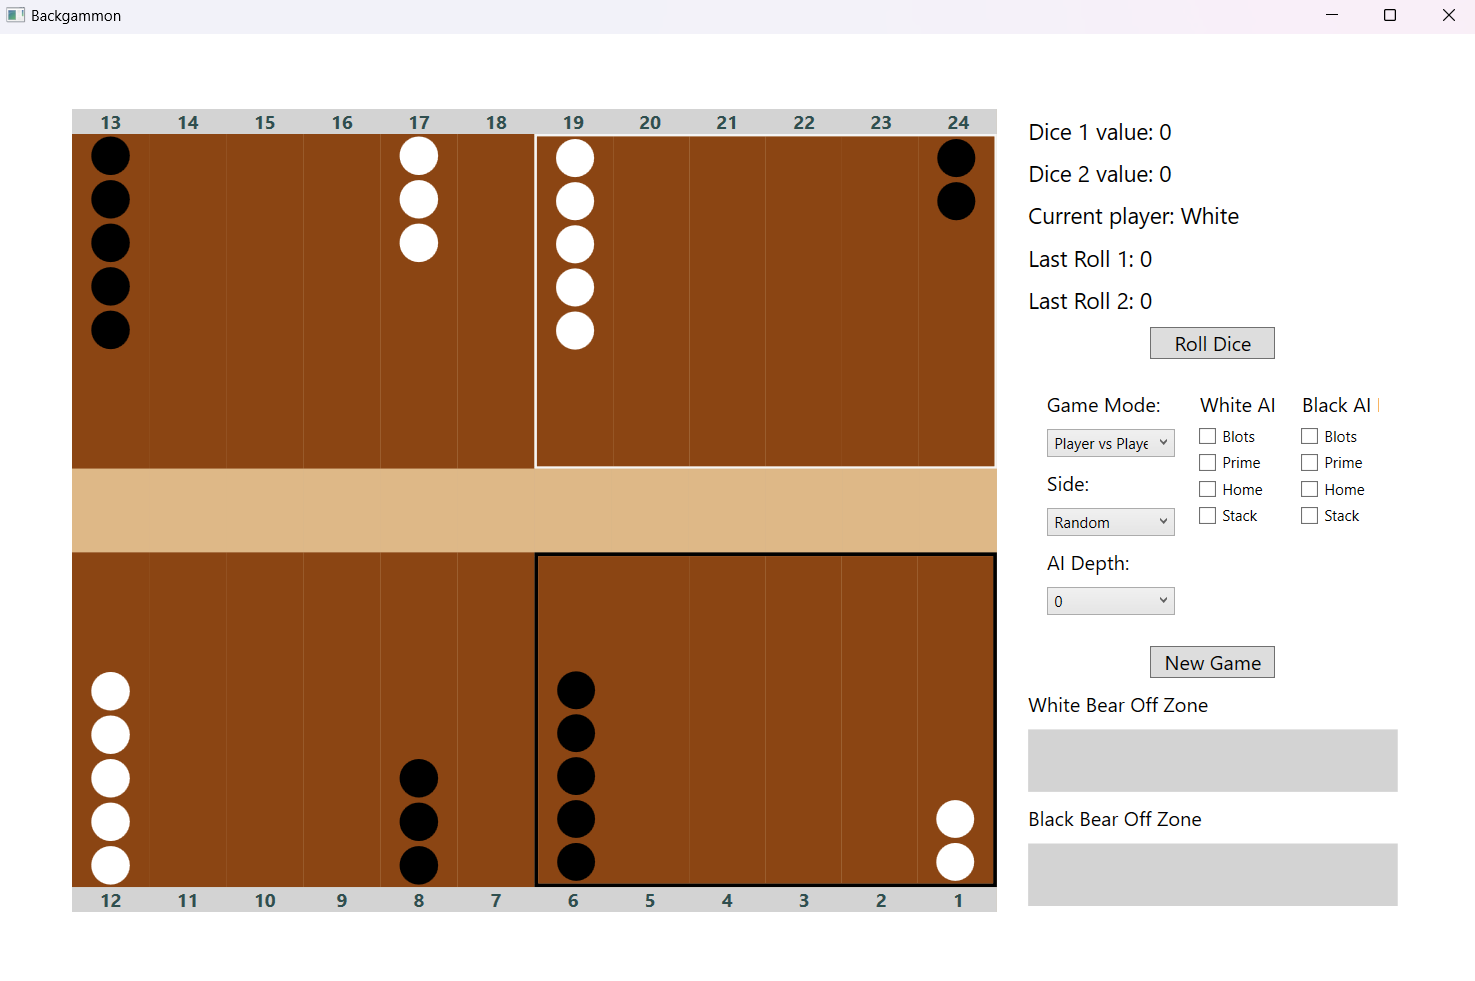
\includegraphics[width=0.9\linewidth]{obrazky-figures/Backgammon_initial_setup.png}
    \caption{User interface of the Backgammon. Initial setup}
    \label{InitialSetup}
\end{figure}

The figure \ref{InitialSetup} shows the board on the left side with 24 numbered points, where checkers are placed and moved. The middle bar serves as the holding area for checkers sent to it. The two bear-off zones are at the bottom right, showing removed checkers for the white and black players. On the right side of the window, various controls are available: dice roll values, current player indicator, last roll memory, and the "Roll Dice" button. Dropdowns and checkboxes allow players to select game mode, AI behavior, playing side, and search depth for the AI. The "New Game" button resets the game state and returns the board to its initial setup. The only significant difference is that the bar on the classic board divides it in half vertically, while in this implementation, it is horizontal. To separate the home points from the outside points, the home points have borders with a color depending on the player to whom they belong.


\begin{figure}[H]
    \centering
    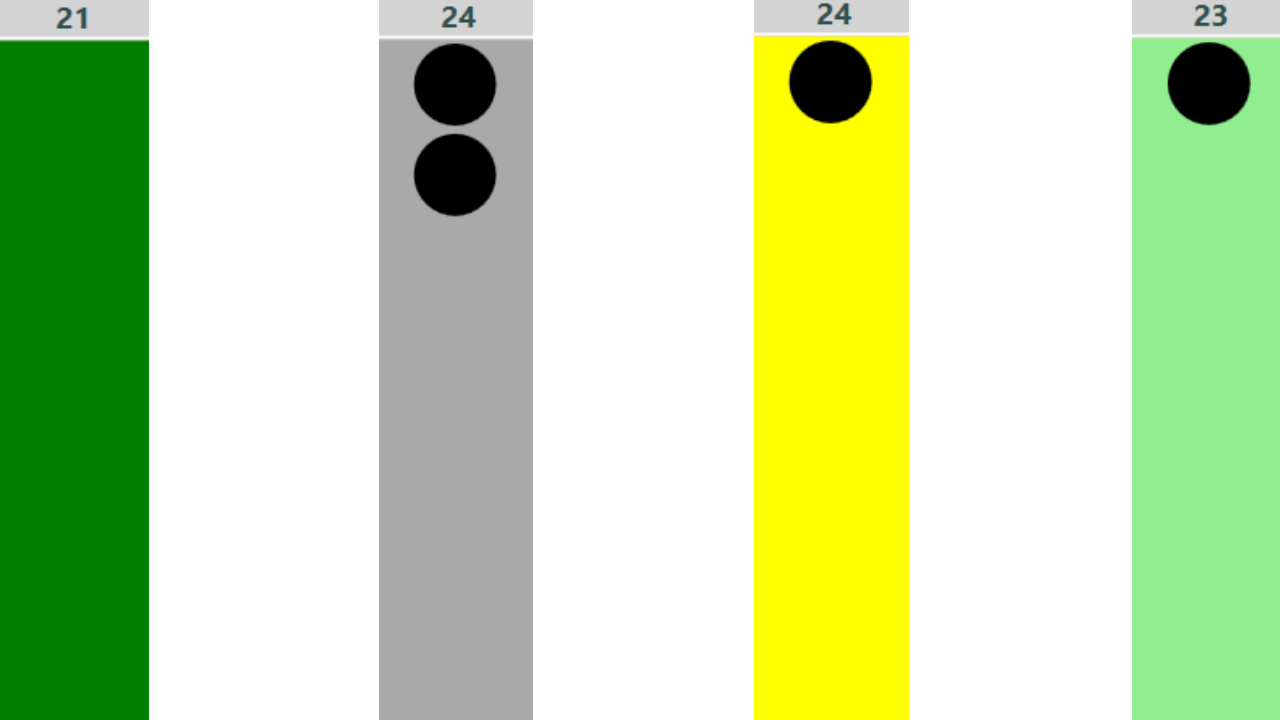
\includegraphics[width=0.5\linewidth]{obrazky-figures/Highlight.png}
    \caption{Highlighting points}
    \label{fig:highlight}
\end{figure}
An important visual aid in the user interface is the move highlighting feature. When a player selects a checker, the point it is located on is highlighted in gray, and all valid destination points are highlighted in green. This helps the player easily identify legal moves based on the current dice roll. The available destinations are calculated using Core and displayed in the UI. The highlights are reset after the move is completed or cancelled.

The figure ~\ref{fig:highlight} illustrates several types of point highlights used during a player's turn, presented from left to right:

\begin{enumerate}
    \item A point that represents a valid destination for the currently selected point, based on the current unused dice values.
    \item The currently selected point by the player.
    \item The point from which a checker has already been moved during the current turn.
    \item The point to which a checker has already been moved within the same move sequence.
\end{enumerate}

\section{Artificial Intelligence}

The artificial intelligence (AI) system is designed to simulate a competitive opponent in Backgammon. Its primary goal is to evaluate the current state of the game, anticipate future possibilities, and make decisions that maximize its chance of winning. The AI interacts directly with the core game logic and follows the same rules as a human player, including dice-based randomness and legal move constraints. This section describes the internal architecture of the AI component and the implementation of the ExpectiMiniMax algorithm that enables intelligent decision-making.

\subsection{AI Player Architecture}

The AI is implemented as a dedicated class within the \texttt{Core} library and is initialized with a reference to the game board and the player it represents. It is constructed with awareness of both players and operates independently of the user interface. The AI is engaged automatically during its turn and does not require direct user interaction.

To make decisions, the AI receives the current game state and dice roll, and generates all possible move sequences available to it using method \texttt{GenerateUniqueStates}. The core method responsible for this is \texttt{GetBestMove}, which returns a list of moves that represents the optimal strategy based on the current state. Internally, this method calls the Expecti\-Mini\-Max algorithm to evaluate various future outcomes and select the path with the highest expected value.

The AI supports configurable evaluation functions by combining multiple scoring factors which will be discussed in detail in Chapter~\ref{Evaluation}. The factors are applied dynamically during the evaluation of game states. Once the best sequence of moves is determined, the game executes them using the same mechanics as for a human player.

\subsection{ExpectiMiniMax Implementation}

The AI player makes decisions by simulating the game multiple steps ahead, taking into account both deterministic actions and stochastic elements introduced by dice rolls. Its behavior is driven by the ExpectiMiniMax algorithm, which evaluates possible move sequences and selects the one with the highest expected utility. The full decision-making process of the AI player consists of the following steps:

\begin{enumerate}
    \item Explore all legal actions based on the current dice values.
    \item Simulate all resulting board states and store them in a searchable structure.
    \item For each resulting state, simulate the opponent's potential responses based on all possible dice outcomes.
    \item For each of those opponent responses, simulate the AI's potential replies using another level of ExpectiMiniMax.
    \item Evaluate the final states using a configurable evaluation function based on heuristic factors.
    \item Select and return the initial move sequence that leads to the highest expected outcome.
\end{enumerate}

In the following subsections, each part of the algorithm will be described in more detail, starting with the entry point of the process.

\subsubsection{GetBestMove}\label{GetBestMove}

The method \texttt{GetBestMove} serves as the entry point for the AI decision process. It is called at the beginning of the AI's turn and receives two parameters: the current dice values (already rolled) and the search depth. This method is responsible for generating and evaluating all possible outcomes that the AI can reach using the current dice.

The first step performed by \texttt{GetBestMove} is to generate all unique game states that can be reached by the AI player, given the current dice values. This is achieved through the method \texttt{GenerateUniqueStates}, which explores different move sequences by recursively applying valid moves and simulating their results on cloned copies of the board. For each unique resulting state, a move sequence is recorded and associated with a hashed representation of the board.

Once all reachable states are collected, the algorithm sorts them to prioritize states where the opponent has more checkers on the bar. This is based on the assumption that hitting checkers is often beneficial and may limit the opponent's responses.

For each resulting state, the method calls \texttt{ExpectiMiniMax} recursively. This function explores future outcomes, alternating between AI and opponent moves while handling dice randomness. After evaluating all possible outcomes, \texttt{GetBestMove} returns the move sequence that leads to the state with the best evaluation score.

Internally, all move sequences are stored in a dictionary called \texttt{stateToMoves}, which maps hashed board states to their corresponding move sequences. Once the best end state is found, the actual moves are retrieved using \texttt{RetrieveMoveSequence} and executed by the AI in order.

\subsubsection{GenerateUniqueStates}\label{GenerateStates}

The method \texttt{GenerateUniqueStates} is responsible for generating all possible board states that the AI player can reach from a given starting board and dice values. This function is essential for expanding the game tree at each ply, as it explores every unique move sequence available to the player.

The method works recursively and operates on cloned copies of the current board. At each level of recursion, it attempts to apply every valid move using the current dice values. Each time a move is simulated, the function calls itself again with the resulting board and the remaining dice values. This process continues until no further moves can be made or all dice have been used.

\begin{figure}[H]
    \centering
    \begin{tikzpicture}[
  every node/.style={draw, circle, minimum size=1cm, font=\small},
  ->, >=Stealth
]

% Main node
\node (A) at (0,0) {[3,5]};

% Children
\node (B1) at (-4,-2) {[5]};
\node (B2) at (-2,-2) {[3]};
\node (C1) [draw=red, double, double distance=1pt] at (-3, -4) {[$\emptyset$]}; % Double red border
\node (B3) at (0,-2) {[3]};
\node (B4) [draw=red, double, double distance=1pt] at (2,-2) {[5]}; % Double red border
\node (C2) [draw=red, double, double distance=1pt] at (2,-4) {[$\emptyset$]}; % Double red border
\node (B5) at (4,-2) {[5]};

% Edges
\foreach \i in {1,2,3,4,5} {
  \draw (A) -- (B\i);
}
\draw (B1) -- (C1);
\draw (B2) -- (C1);
\draw (B3) -- (C2);
\draw (B5) -- (C2);

% Caption under B4
\node[draw=none, font=\footnotesize, inner sep=0pt] at ($(B4)+(0,-0.8)$) {No legal moves};

\end{tikzpicture}
    \label{Permutations}
    \caption{Permutations}
\end{figure}
Many states are the same and result from different permutations of moves. The player can move in a different order and reach the same state.
This is shown in Figure \ref{Permutations}. Each graph node represents a separate game state; the end states are marked. The game's initial state (the root node) has two unused dice values. Its child nodes represent the states after one dice value is used. It makes no sense to evaluate them immediately, since they lead to a common end state where all dice values are used. For any dice value that is not a double (as in the figure, where dice have different values), the number of states leading to one common state is $2! = 2$, for doubles this value is higher and in the worst case reaches $4! = 24$. The task of the method is to extract only the final states (i.e., states where all dice values are used or there are no legal moves).
All such game states are stored in a separate dictionary, where each corresponds to a sequence of moves that leads to it. A state is a complex structure that occupies a relatively large amount of memory space. At the same time, hundreds of thousands of such states must be stored. In this case, using a hash table is much more efficient. Such tables are called transposition tables and are widely used in this algorithm.

The algorithm uses a hashing mechanism to ensure that only unique states are explored. Each board state is represented as a string key generated by the \texttt{HashBoardState} method. This key includes:
\begin{itemize}
    \item The index of each point on the board that has at least one checker.
    \item The number of checkers on this point.
    \item The owner's color.
    \item The number of checkers on each player's bar.
\end{itemize}

For example, there is a point with index 5, which has 2 black checkers on it. Such point is represented as \texttt{5:2:B} representing \texttt{index:quantity:color}. Points are separated by '|' symbol. So the whole key has the following format:
$$
\texttt{1:2:W|2:1:B|6:4:B|8:2:B|12:5:W|13:5:B|17:3:W|19:5:W|24:2:B|0:WBar|0:BBar}
$$

Of course, it is possible to shorten this key, but the current structure makes it very easy for a human to read and reproduce positions, and does not take up too much memory. As the recursive process explores new states, each hashed state is added to a dictionary called \texttt{stateToMoves}. This dictionary maps the hashed key to the corresponding move sequence in the format \texttt{\{int src, int dst\}} that produced the state. This prevents redundant computation and guarantees that different sequences leading to the same result are not re-evaluated. .NET uses UTF-16 encoding \cite{microsoft_utf16}, so each char in the key takes 2 bytes. Thus, each new key-value pair in the dictionary takes about 220-240 bytes, so an entire dictionary for 3-ply search rarely takes more than 350-400MB of memory.

If a state has already been encountered (i.e., its hash exists in the dictionary), it is skipped. This technique significantly reduces the number of states the AI needs to consider and optimizes the decision process without compromising correctness.

By the end of the method, the AI has a list of unique resulting board states, each associated with a valid sequence of moves. These states serve as candidates for further evaluation by the ExpectiMiniMax algorithm.

\subsubsection{ExpectiMiniMax and MinimaxForDiceOutcome}

The method \texttt{ExpectiMiniMax} is the core of the AI's decision-making process. It is a recursive function that evaluates the expected value of a game state and simulates all possible outcomes that may occur due to dice rolls and player responses. This method extends the traditional MiniMax algorithm and handles stochastic elements of Backgammon. These chance nodes represent all possible dice outcomes that could occur on a player's turn.

Unlike standard MiniMax, which evaluates a single deterministic move per player per ply, \texttt{ExpectiMiniMax} evaluates every possible combination of dice rolls. In the context of Backgammon, there are 21 unique outcomes of rolling two six-sided dice, including 15 non-doubles (each occurring twice due to symmetry) and six doubles (each occurring once). As a result, each level of the ExpectiMiniMax tree performs up to 21 independent evaluations of potential outcomes.

This structure effectively generalizes the MiniMax algorithm by calling it 21 times per ply. At each call, the function \texttt{MinimaxForDiceOutcome} is used to perform a standard MiniMax evaluation for a specific dice combination.


\begin{algorithm}[H]
\caption{ExpectiMiniMax Algorithm}
\label{expectiminimaxImplemented}
\begin{algorithmic}[1]
\Function{ExpectiMiniMax}{$board$, $depth$, $maximizingPlayer$, $currentPlayer$}
    \State $diceOutcomes \gets$ \Call{GenerateAllDiceOutcomes}{}
    \State $totalValue \gets 0$
    \State $totalFrequency \gets 0$

    \For{each $dice$ in $diceOutcomes$}
        \State $frequency \gets$ \Call{OutcomeFrequency}{$dice$}
        \State $value \gets$ \Call{MinimaxForDiceOutcome}{$board$, $depth$, $maximizingPlayer$, $currentPlayer$, $dice$}
        \State $totalValue \gets totalValue + (frequency \times value)$
        \State $totalFrequency \gets totalFrequency + frequency$
    \EndFor

    \If{$totalFrequency = 0$}
        \State \Return \textbf{if} $maximizingPlayer$ \textbf{then} $-\infty$ \textbf{else} $+\infty$
    \EndIf

    \State \Return $totalValue / totalFrequency$
\EndFunction
\end{algorithmic}
\end{algorithm}

The Algorithm \ref{expectiminimaxImplemented} represents the real algorithm used in a program as pseudocode. In this algorithm:

\begin{itemize}
    \item \texttt{diceOutcomes} is a list of all possible dice rolls in Backgammon. It contains 21 unique outcomes, including both doubles (e.g., 4--4) and non-doubles (e.g., 2--5), which are generated by the helper function \texttt{GenerateAllDiceOutcomes}.
    
    \item \texttt{totalValue} is a variable used to accumulate the weighted sum of all evaluation values across different dice outcomes.
    
    \item \texttt{totalFrequency} keeps track of the total weight, or count, of all evaluated outcomes. For example, non-doubles occur with frequency 2 due to symmetry, while doubles occur with frequency 1.
\end{itemize}

\subsubsection{MiniMax for Dice Outcome}

The method \texttt{MinimaxForDiceOutcome} is a helper function used within the ExpectiMiniMax algorithm. While \texttt{ExpectiMiniMax} is responsible for handling uncertainty through chance nodes (dice rolls), this method performs the actual deterministic evaluation for a single dice outcome. It operates in the same way as a classical MiniMax algorithm, alternating between minimizing and maximizing players.

The method begins by generating all unique board states that the current player can reach using the specified dice outcome. These are obtained using the \texttt{GenerateUniqueStates} method, which simulates all legal move sequences and avoids duplicate states using hashing.



\begin{algorithm}[H]
\caption{Minimax for Dice Outcome}
\label{alg:minimaxfordice}
\begin{algorithmic}[1]
\Function{MinimaxForDiceOutcome}{$board$, $depth$, $maximizingPlayer$, $currentPlayer$, $dice$}
    \State $states \gets$ \Call{GenerateUniqueStates}{$board$, $currentPlayer$, $dice$}

    \If{$states$ is empty}
        \State $penalty \gets$ \Call{EvaluateBoard}{$currentPlayer$, $board$}
        \State $penalty \gets$ \textbf{if} $maximizingPlayer$ \textbf{then} $penalty - 10$ \textbf{else} $penalty + 10$
        \State \Return $penalty$
    \EndIf
\State $opponent \gets$ \Call{GetOpponent}{$currentPlayer$}
    \If{$maximizingPlayer$}
        \State $value \gets -\infty$
        \For{each $state$ in $states$}
            \State $childValue \gets$ \Call{ExpectiMiniMax}{$state\, depth-1\, \textbf{false}, opponent$}
            \State $value \gets \max(value, childValue)$
            \If{$value \geq \beta$}
                \State \Return $value$ \Comment{$\beta$ cutoff}
            \EndIf
            \State $\alpha \gets \max(\alpha, value)$
        \EndFor
        \State \Return $value$
    \Else
        \State $value \gets +\infty$
        \For{each $state$ in $states$}
            \State $childValue \gets$ \Call{ExpectiMiniMax}{$state$, $depth-1$, \textbf{true}, $opponent$}
            \State $value \gets \min(value, childValue)$
            \If{$value \leq \alpha$}
                \State \Return $value$ \Comment{$\alpha$ cutoff}
            \EndIf
            \State $\beta \gets \min(\beta, value)$
        \EndFor
        \State \Return $value$
    \EndIf
\EndFunction
\end{algorithmic}
\end{algorithm}

The components of the algorithm work as follows:

\begin{itemize}
    \item The call to \texttt{GenerateUniqueStates} produces all valid game states reachable from the current board. If the \texttt{states} list is empty, it means that the player has no legal moves available. In this case, the algorithm applies a penalty to simulate the negative impact of skipping a turn.

    \item The variable \texttt{opponent} stores the opposing player, whose turn will follow next in the recursion.
\end{itemize}

The algorithm returns the best score found among all child states, depending on whether it is a maximizing or minimizing level.

The important part is that if no legal moves are found, it is treated as a skipped turn. In this case, the current evaluation of the board is calculated, which will be discussed in more detail in Section \ref{Evaluation}. Rather than returning a neutral value, the algorithm applies a small penalty to reflect the disadvantage of losing a move. On average, a Backgammon player advances approximately 8.166 points per move (more detailed in Appendix \hyperref[avg_pips]{B}). Additionally, skipping a move may expose checkers to hits by the opponent. Therefore, a rounded penalty of 10 points is applied to simulate the impact of missing a turn.

If legal moves are available, the method recursively calls \texttt{ExpectiMiniMax} on each resulting board state, switching the player role (from maximizing to minimizing or vice versa). The method uses Alpha-Beta pruning, which is reflected in the pseudocode.

After evaluating all possible resulting states using the ExpectiMiniMax algorithm, the AI selects the one with the highest expected value. Each board state is associated with a unique move sequence, which was stored earlier during move generation using the \texttt{stateToMoves} dictionary. This dictionary maps hashed representations of board states to the exact sequence of moves that led to them. Once the best board state is identified, the AI retrieves the corresponding move sequence using the \texttt{RetrieveMoveSequence} method.

The evaluation itself is performed using a separate evaluation function, which returns an integer value estimating how favorable a given game state is for the current player. The details and structure of this evaluation function will be discussed later in Chapter~\ref{Evaluation}.

Finally, the move sequence is executed step-by-step using the same public methods as would be called for a human player. This ensures full compliance with game rules and allows the AI to play transparently within the existing game loop. Each move is processed using the same validation and board update routines, so it preserves consistency between AI and user interactions.


\chapter{Optimizations of ExpectiMiniMax}\label{Optimizations}


The ExpectiMiniMax algorithm is computationally intensive due to its recursive nature and the many possible game states that need evaluation. Since each ply expands into multiple branches depending on all possible dice outcomes, the number of states grows exponentially with the search depth. In practice, this makes the algorithm slow to compute and demanding regarding memory usage. For example, *-MiniMax algorithm is much more optimized and can search at a depth of 5 plies, but it requires normalization of the evaluation function \cite{*-MiniMax}.

The total computation time depends on two key factors: the number of game states that need evaluation and the time it takes to evaluate a single state. Several optimization strategies were introduced to make the AI responsive and usable during gameplay. These strategies focus on reducing the number of states to process, speeding up state evaluation, and better using hardware capabilities such as multithreading.

This chapter discusses the main optimizations applied in the implementation. Each subsection presents a different approach to improving performance.

\section{Time Complexity and the need for optimization}

Each decision made by the AI involves simulating many possible future states, which increases rapidly with the depth of the search.

In Backgammon, a single move by a player is influenced by the outcome of two dice. There are 21 unique dice outcomes when considering symmetrical values and doubles. The number of legal game states a player can reach for each outcome varies, but in practice, it averages around 19-20 states per outcome. Thus, for one ply (i.e., one player's complete move), the number of possible resulting game states can be estimated as:

\[
N_1 = 21 \times 20 = 420
\]

When evaluating a depth of 3 plies — one move by the AI, one move by the opponent, and one additional response by the AI — the number of game states to explore grows multiplicatively at each level. Assuming similar branching factors at each ply, the total number of states can be estimated as:

\[
N_{\text{total}} = (21 \times 20)^3 = 420^3 = 74,\!088,\!000
\]

This means that to fully evaluate the game tree at a depth of 3 plies, the algorithm may need to process over 74 million distinct board states, each requiring move generation, simulation, and evaluation. This computational cost makes real-time decision-making nearly impossible without additional optimizations. In practice, the number of states reaches about 5 million, and the calculation time reaches 9 minutes.

Furthermore, for each terminal node (leaf) in the tree, a numerical evaluation must be calculated using the heuristic evaluation function. Since this function is called once per leaf node, and potentially hundreds of thousands of times during the complete evaluation, its performance has a significant impact on the overall runtime of the AI.

Due to this exponential time complexity, it is essential to implement various optimization techniques to reduce the number of states considered and speed up individual computations. These techniques — such as alpha-beta pruning, state caching, and multithreading — are discussed in the following sections.

\section{Search Tree Pruning with State Sorting}

In the MiniMax algorithm, it is not necessary to explore all branches, skipping some of them can reduce the search time without changing the result. The technique of cutting off unnecessary branches is called \textbf{Alpha-Beta pruning}. \cite[Section 5.3]{russel2010}

\begin{figure}[H]
    \centering
    \begin{tikzpicture}[
      maxnode/.style={regular polygon, regular polygon sides=3, shape border rotate=0, draw, fill=blue!15, minimum size=1.2cm, font=\small},
      minnode/.style={regular polygon, regular polygon sides=3, shape border rotate=180, draw, fill=red!15, minimum size=1.2cm, font=\small},
      leafnode/.style={circle, draw, minimum size=1cm, font=\small, fill=gray!10},
      pruned/.style={draw=none, font=\small},
      ->, >=Stealth
    ]

    % Level 1 (MAX)
    \node[maxnode] (A) at (0,0) {5};

    % Level 2 (MIN)
    \node[minnode] (B1) at (-4,-2) {1};
    \node[minnode] (B2) at (0,-2) {-3};
    \node[minnode] (B3) at (4,-2) {5};

    % Level 3 (MAX/Leaf)
    \node[leafnode] (C1) at (-5.5,-4) {3};
    \node[leafnode] (C2) at (-4,-4) {1};
    \node[leafnode] (C3) at (-2.5,-4) {5};

    \node[leafnode] (C4) at (-1,-4) {-3};
    \node[leafnode] (C6) at (1,-4) {2}; % PRUNED

    % Edges from root to MINs
    \draw (A) -- (B1);
    \draw (A) -- (B2);
    \draw (A) -- (B3);

    % Edges for first MIN subtree
    \draw (B1) -- (C1);
    \draw (B1) -- (C2);
    \draw (B1) -- (C3);

    % Edges for second MIN subtree
    \draw (B2) -- (C4);
    \draw[dashed, red] (B2) -- (C6); % Pruned edge

    % Labels for levels
    \node[draw=none, font=\footnotesize, gray] at (-1.2, 0) {MAX};
    \node[draw=none, font=\footnotesize, gray] at (-5, -2) {MIN};
    \node[draw=none, font=\footnotesize, gray] at ($(C1)+(-1,0)$) {MAX};

    % Red X on pruned node
    \node[pruned] at ($(C6)+(-0.5,1)$) {\textcolor{red}{\Large$\times$}};

    \end{tikzpicture}
    \caption{Alpha-Beta Pruning example}
    \label{fig:alpha-beta-diagram}
\end{figure}

The tree in Figure~\ref{fig:alpha-beta-diagram} illustrates how Alpha-Beta pruning operates on a three-level game tree with alternating MAX, MIN, and MAX players.

At the root, which is a MAX node, the algorithm begins with initial values of $\alpha = -\infty$ and $\beta = +\infty$. It first explores the leftmost MIN subtree. This MIN node has three children, each representing a possible MAX move that returns a value of 3, 1, and 5, respectively. MAX uses these to update its internal $\alpha$ value. After processing all children, MIN selects the minimum among them, which is 1, and returns it to the root. The root MAX node then updates its current best value to $\alpha = 1$.

Next, the algorithm moves to the second MIN subtree. Its first child (a MAX node) evaluates to $-3$, so MIN's current best value becomes $-3$, and $\beta$ is updated accordingly. However, before evaluating the second child of this MIN node, the algorithm checks whether further exploration is necessary. Since the current MIN value $v = -3$ is already less than or equal to $\alpha = 1$ (MAX's best so far), the second child is immediately pruned. There's no need to evaluate it because MAX would never choose a path that allows the opponent to force a result worse than what has already been seen (the leftmost child with value 1).

After pruning, the algorithm proceeds to the final MIN subtree on the right, which contains a single MAX node returning 5. This value is passed back up to the root, and MAX compares it with the previous best value. Since 5 is greater than 1, MAX updates its final result to 5.

As shown in this example, Alpha-Beta pruning allowed the algorithm to skip evaluating a portion of the tree without affecting the outcome. The key decision to prune was based on the inequality $v \leq \alpha$, where the current MIN value could not possibly result in a better outcome for the MAX player. This makes Alpha-Beta pruning an essential optimization for efficient adversarial search. 


\subsection{Sorting moves}
The Alpha-Beta pruning is not a consistent technique. At best, the time complexity of the algorithm will be $O(\sqrt{b^m})$. At the same time, in the worst-case scenario, the time complexity will not differ from the classic MiniMax. Alpha-Beta pruning is very sensitive to the order of moves. From the perspective of the MAX node, if the leftmost child has a high value (probably a good move), then most of the following branches will be cut off, and the algorithm will approach the time complexity of the best-case scenario.

Therefore, before evaluating the generated game states, it is necessary to sort them so that the most promising moves are evaluated first. Such moves should give a strategic advantage at least at first glance. The principle by which the moves are sorted should not be too complicated. There is no point in evaluating a move very well if it is evaluated well at the maximum depth, as this will only slow down the algorithm and negate the point of sorting. A relatively simple way that has been implemented is to evaluate first of all \textbf{moves where the current player has beaten the enemy's checker}. This makes good use of the subsequent evaluation function that considers the distance of the checkers to the edge of the board. These moves are not always good, as they sometimes open up a position for the opponent's counterplay, but they are enough to cut out most moves that do not provide any strategic advantage in the future.

In general, only the use of Alpha-Beta pruning made it possible to reduce the number of states to be evaluated by 10-12 times compared to the unoptimized version in the current implementation of the game. The search time has decreased to 1 minute per move for a 3-ply game, which is still unreasonably a lot and requires further optimizations.

\section{Optimizations for evaluation function}

The evaluation function plays a critical role in the ExpectiMiniMax algorithm, as it determines the heuristic value of a game state when the search reaches a leaf node. Due to the branching factor and multiple dice outcomes in Backgammon, the evaluation function can be executed hundreds of thousands or even millions of times during a single decision cycle. Therefore, optimizing this function is essential for maintaining reasonable performance. The task of optimization is to shorten the code as much as possible and avoid various factors that affect the speed of its execution.
\newpage
It is possible to find some key considerations for optimizing the evaluation function in C\#:

\begin{itemize}
    \item \textbf{Avoiding high-level constructs.}
    For example, \texttt{foreach} is readable and has very clean syntax, but it introduces iterator overhead, especially when applied to arrays. It is much better to replace this construct with a traditional \texttt{for} loop—such as \texttt{for (int i = 0; i < 24; i++)}. It eliminates the creation of an enumerator object and improves performance.

    \item \textbf{Reducing repeated property access.} 
    Assigning frequently accessed properties to local variables, such as caching \texttt{board.Points} into a \texttt{var points} reference, reduces function call overhead and avoids redundant property access within loops.

    \item \textbf{Avoiding unnecessary allocations.} 
    Such features like LINQ introduce hidden allocations and delayed execution. In performance-critical code, it is better to prevent redundant memory usage.

\end{itemize}

This problem applies to high-level programming languages, and it's necessary to be as efficient as possible when writing such critical code.

\paragraph{Example: Evaluating Board Distance}

\begin{verbatim}
for (int i = 0; i < 24; i++)
{
    var point = board.Points[i];
    if (point.Owner == CheckerColor.White)
        whiteDistance += (25 - i) * point.Checkers.Count;
    if (point.Owner == CheckerColor.Black)
        blackDistance += i * point.Checkers.Count;
}
\end{verbatim}

The code snippet is a part of the implemented evaluation function, which computes total checker distances for each player.

Conditional statements inside tight loops—especially nested \texttt{if-else} blocks—introduce branches that can disrupt the processor's ability to predict upcoming instructions. Modern CPUs rely heavily on branch prediction to avoid pipeline stalls. If the branch condition is unpredictable (e.g., changes frequently between iterations), the CPU mispredicts and flushes the pipeline, causing performance penalties. It is important to use such conditional statements as little as possible. Also, if some value is a known constant, for example, the number of points on the board, it is much better to use a constant number instead of calling the same function \verb|point.Count()|.

Since the evaluation function is called so frequently, optimizing even small parts of it can produce significant performance gains. These micro-optimizations have a cumulative effect and collectively enable the AI to calculate the optimal move much faster. The saved time depends on the complexity of the evaluation function itself, so this function should be as simple as possible for the fastest execution.

\newpage
\section{Parallel Processing of Dice Outcomes}
The following optimization was inspired by and partially based on \cite{Lamanosa2013ExpectimaxET}.

In the ExpectiMiniMax algorithm, all dice outcomes are modeled as chance nodes, and their child nodes represent all possible responses to a specific dice roll.

Since the result of one dice outcome does not affect the others, these branches of the search tree are mutually independent. As a result, the evaluation of each dice outcome can be performed in parallel. This idea is implemented in the \texttt{ExpectiMiniMax} method by launching a separate task for each of the 21 dice outcomes. These tasks compute the expected value for each chance node concurrently.

\begin{itemize}
    \item Each task executes the method \texttt{MinimaxForDiceOutcome}, which performs a full minimax evaluation for a single dice roll.
    \item All tasks are collected into a list and executed in parallel using \texttt{Task.Run()}.
    \item After all tasks complete, the weighted average of their results is used to compute the final expected value.
\end{itemize}

This parallelism allows the AI to utilize multiple processor cores and significantly reduces the time required to process deep trees, especially when the number of states grows exponentially with search depth.

\begin{figure}[H]
    \centering
    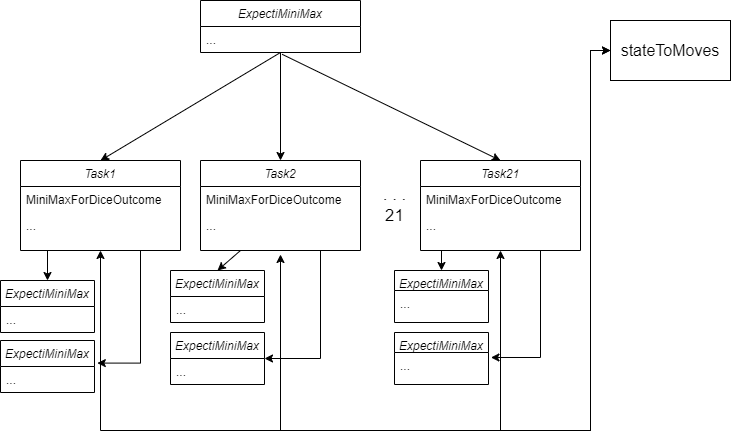
\includegraphics[width=1\linewidth]{obrazky-figures/tasks.drawio.png}
    \caption{Tasks structure}
    \label{tasks}
\end{figure}

The figure \ref{tasks} shows a diagram of the relationship structure between the Expecti\-Mini\-Max and MiniMax methods, where each MiniMax is in its own task. This method uses the stateToMoves dictionary to read and write new hashed states of the board. MiniMax methods call ExpectiMiniMax, which in turn can also create new tasks.
\newpage
This structure leads to certain problems, so it must be implemented very carefully. The biggest problems are:

\begin{itemize}
    \item \textbf{Shared memory} \\
    Although this technique significantly speeds up computations, it should be implemented with caution, as such asynchronous processes are quite dangerous when working with shared memory. ExpectiMiniMax uses three such memory locations: Alpha, Beta, and the stateToMoves dictionary. Alpha and Beta change relatively rarely, unlike the dictionary, where each task constantly reads it and writes new hashed states. To prevent conflicts, it is implemented as a \texttt{ConcurrentDictionary}, which ensures thread-safe access. 

    \item \textbf{Number of tasks} \\
    Creating new tasks inside recursive methods with increased caution is necessary as the number grows exponentially. The best solution is to use them in one or a maximum of two deepest levels of the tree. Involving more levels will create an absurdly large number of tasks, and making them near the tree's root will artificially make the breadth-first search tree and eliminate the essence of Alpha-Beta and MiniMax, which requires a depth-first search tree.
\end{itemize}

With this kind of task usage, shared memory becomes a bottleneck, as tasks still need to wait for their turn to write new data and cannot run completely separately. Nevertheless, this effect is relatively moderate and has little effect on the speed of computation. Limiting the ability to create new tasks at the last two levels of the tree, the average number of tasks will be about 100; it will never reach $21^2$. Generating new board states and hashing them takes relatively more time than writing to the dictionary. The keys are guaranteed to be unique for almost all cases. The only exception is the late game, when any player bears off checkers. In this situation, the branching factor is minimal, so even trying to write the same key with different tasks does not have an adverse effect on the speed.


\section{Selective deepening}

Sorting moves by their degree of benefit and strategic impact helps the Alpha-Beta pruning technique to cut off significantly larger parts of the tree and do so more often, but at the same time, this approach implies traversing all branches of the tree. For additional optimization and to reduce the number of nodes to be examined, the selective deepening method can be used. Very similar idea was described by Buro and applied to the game Othello. His ProbCut~\cite{buro1995probcut} method proposes statistical pruning based on shallow evaluation predictions.

The core idea behind the proposed optimization is to exploit the observation that, in practice, strong human players do not evaluate every possible move uniformly. Instead, they instinctively focus on moves that appear more promising based on experience and board intuition. Intuition is a rather vague concept, so it must be replaced by a heuristic algorithm for sorting possible moves. Translating this to a computational model, the algorithm sorts available moves using a heuristic evaluation function and assumes that better moves are more likely to appear earlier in the list. By evaluating only a subset of these top-ranked moves—typically the left half of the move list—significant parts of the search tree can be pruned, resulting in a reduction in node count.

\newpage
The logic of the approach can be described in the following steps:

\begin{enumerate}
    \item Use a heuristic function to sort available moves so that more promising ones appear first in the list.
    \item Simulate a large number of games and analyze in which part of the move list the best move usually appears. Choose a cutoff percentile that captures the best moves most of the time.
    \item During actual search, explore only moves within the selected top percentile, and ignore the rest. This reduces the number of nodes the algorithm has to evaluate.
\end{enumerate}

This approach works similarly to beam search, where only a limited number of best candidates are expanded. It does not guarantee that the best move will always be considered, but it allows the algorithm to search more deeply in promising areas.
It can make the algorithm run much faster by reducing the number of moves it looks at during search. Because the algorithm does not spend time on clearly weak moves, it can go deeper into the game tree. This may help it find better long-term strategies. The cutoff point for pruning can be based on real data from simulated games, which makes the decision more informed instead of being based on guesswork.

 Nevertheless, this approach has weaknesses:

 \begin{itemize}
     \item  The method does not look at every possible move, so it might miss important moves that are not ranked highly by the heuristic. This can lead to mistakes if the heuristic is not reliable. If the move sorting works well near the root of the tree but gets worse deeper down, the search may become weaker the further it goes.
     \item The best cutoff percentile may change depending on the phase of the game or the situation on the board, so tuning it once might not work well for all positions.
 \end{itemize}



Although this method does not follow the standard minimax logic strictly, it can be a useful tradeoff between accuracy and speed. In situations where quick decisions are more important than perfect accuracy, this technique may offer a practical advantage.

This topic is controversial and requires much more research, so this approach was not implemented. The technique is based on the fact that there exists a certain heuristic algorithm that will accurately eliminate all “weak” moves. Assuming that such an algorithm already exists, applying it to the Alpha-Beta pruning will bring it as close as possible to the best-case time complexity. If so, how much faster will the search be by ignoring some of the branches compared to the Alpha-Beta pruning? If there is no such heuristic algorithm, then ignoring the branches may result in missing out on a win. In general, this approach may be implemented after deeper research and will possibly allow ExpectiMiniMax to work at 4-ply depth.

\chapter{Evaluation function, factors that impact the game}\label{Evaluation}

\section{Evaluation Function}
The evaluation function is the most important part of the ExpectiMiniMax algorithm. It doesn't matter how deeply search goes, or how fast states are evaluated, if the evaluation function does not evaluate positions well and does not reflect the real situation on the board. The ExpectiMiniMax algorithm has known limits, so practically the only way to improve its quality is to create the best possible evaluation function.


In adversarial game AI, the evaluation function estimates how favorable a given board state is for a player when the search reaches a non-terminal node. In the ExpectiMiniMax algorithm, this function is invoked at the leaf nodes of the search tree, which means it may be called hundreds of thousands of times during a single move computation. For this reason, it must be both computationally simple and strategically effective. A slow function can become a significant bottleneck, while at the same time, an inaccurate one may lead the AI to misjudge positions consistently.

The evaluation is based on the pip count. A pip count measures the distance a player's checkers must
move to reach their home board and bear off. A lower pip count generally corresponds to a stronger position. The idea of using pip count as a basis for evaluating positions was inspired by the article on Backgammon Galaxy \cite{backgammon_galaxy}, where pip count is used as an indicator of who is ahead in the game. This work extends that concept by formalizing the evaluation as the difference between the player's and opponent's pip totals.

Relying on only one parameter is not a solution, so modular factors extend the evaluation function. These factors adjust the base pip evaluation by accounting for other positional and tactical elements. Each factor can be manually enabled and contributes a multiplicative adjustment to the player's pip-based score. This design enables easy testing of different strategic approaches and evolving the AI's play style without rewriting core logic.

The modularity of this system supports experimenting and performance tuning. Decoupling specific factors from the base evaluation makes it easier to isolate the effects of different strategic components and optimize them independently.

The pip count is calculated for each player by summing the points each checker must advance from its current position to the bearing-off point. For checkers on the bar, the distance to the bear-off point is constant and equals 25. The evaluation function then computes the difference between the opponent's pip count and the current player's pip count. It is possible to formally define the function.

\subsection*{Backgammon Evaluation Function}

Let $B$ denote the current board state, and let $P \in \{\text{White}, \text{Black}\}$ denote the current player.

Define:

\begin{itemize}
    \item $c_i^W$: Number of White checkers on point $i$
    \item $c_i^B$: Number of Black checkers on point $i$
    \item $b^W$: Number of White checkers on the bar
    \item $b^B$: Number of Black checkers on the bar
\end{itemize}

The board consists of 24 points indexed by $i = 1$ to $24$, where:
\begin{itemize}
    \item Point $i = 1$ is closest to home for Black
    \item Point $i = 24$ is closest to home for White
\end{itemize}

\vspace{1em}

\textbf{Pip count for each player:}
\begin{align*}
D_W &= 25 \cdot b^W + \sum_{i=1}^{24} (25 - i) \cdot c_i^W \\
D_B &= 25 \cdot b^B + \sum_{i=1}^{24} i \cdot c_i^B
\end{align*}

Here, $D_W$ and $D_B$ represent the total number of pips (distance to bear off) for White and Black, respectively. The function $E(P, B)$ returns a positive value when player $P$ is in a favorable position (i.e., closer to bearing off), and a negative value when they are behind.

\vspace{1em}

\textbf{Evaluation Function:}
\[
E(P, B) = 
\begin{cases}
D_B - D_W & \text{if } P = \text{White} \\
D_W - D_B & \text{if } P = \text{Black}
\end{cases}
\]



The function is based not only on the number of pips of the current player, but also on the number of pips of his opponent. Since backgammon is a zero-sum game, any increase in the opponent's distance from the board edge indirectly brings the current player closer to winning. Given the fact that any move is the same according to this evaluation, since the checker always moves by the number of dice points given by the dice, the distance to the board edge decreases by the same amount. The difference in choices is made by moves where one player's checker hits another player's checker. The AI chooses moves where it will have the most opportunities to strike in the future, and the opponent will have the least. This provokes the AI to play quite aggressively, which is absolutely the right approach, but at the same time, it is not a guarantee of victory. When the search stops at a certain depth, it does not take into account the potential next moves of the opponent, and strong initial moves can lead to a losing position in the future. It also works vice versa - moderately aggressive moves that create a defensive formation at a certain depth are more stable and usually bring more benefits in the future.

\section{Factors}

\begin{figure}[H]
    \centering
    
    \begin{tikzpicture}[
    node distance=1.5cm and 2cm,
    every node/.style={font=\sffamily, align=center},
    process/.style={rectangle, draw, minimum width=2.8cm, minimum height=1cm, fill=blue!10},
    factor/.style={rectangle, draw, minimum width=2.8cm, minimum height=1cm, fill=green!10, dashed},
    result/.style={rectangle, draw, minimum width=3.2cm, minimum height=1cm, fill=orange!20},
    arrow/.style={-Latex}
]

% Nodes
\node[process] (base) {Base Evaluation \\ (Pip Count)};
\node[factor, above=of base] (f1) {Blot Penalty};
\node[factor, above left=of base] (f2) {Prime Bonus};
\node[factor, left=of base] (f3) {Home Checkers Bonus};
\node[factor, above right=of base] (f5) {Stack Penalty};
\node[factor, right=of base] (f6) {Dead Checkers Penalty};
\node[result, below=2cm of base] (final) {Final Evaluation \\ (Adjusted Score)};

% Arrows from factors to base
\draw[arrow] (f1) -- (base);
\draw[arrow] (f2) -- (base);
\draw[arrow] (f3) -- (base);
\draw[arrow] (f5) -- (base);
\draw[arrow] (f6) -- (base);

% Arrow from base to final
\draw[arrow] (base) -- (final);

\end{tikzpicture}
\caption{Basic evaluation function and main factors}
\end{figure}

The basic evaluation is quite a self-sufficient function, but it has its drawbacks caused by too aggressive play and relatively small search depth. Many different factors influence the strength of a position, so adding them to the basic evaluation strengthens the algorithm and compensates its drawbacks.


The base evaluation function in the AI system for backgammon relies on pip count. While such an evaluation effectively reflects overall game progress, it has a significant drawback: most positions are considered \textbf{equivalent} in pip terms, even if they are strategically very different.

For example, consider a position $A$, from which at depth 3 there are two groups of resulting positions: group $X$, in which the player hits an opponent's checker during the sequence, and group $Y$, in which no checkers are hit. If the evaluation is based solely on pip count, then all positions in group $X$ will have the same score $x$, and all positions in group $Y$ will have the same score $y$. As a result, the system does not recognize the strategic advantage of actions such as building blocks and primes, or avoiding blots and dead checkers.

Furthermore, each move in backgammon often consists of multiple steps that collectively change the board state. Some of these steps may strengthen the position, while others may expose it to risk. Without additional factors, the evaluation function cannot distinguish strong moves from weak ones. This leads to an effect of \textbf{artificial flattening} in the evaluation landscape, which lowers the quality of decisions.

\begin{figure}[H]
    \centering
    \begin{tikzpicture}[
    level distance=2cm,
    sibling distance=1.8cm,
    every node/.style={font=\sffamily},
    root/.style={circle, draw=black, fill=blue!20, minimum size=1cm},
    nodeX/.style={circle, draw=black, fill=green!20, minimum size=1cm},
    nodeY/.style={circle, draw=black, fill=red!20, minimum size=1cm},
    label/.style={font=\sffamily\small}
]

% Root node
\node[root] (A) {A};

% X group (left)
\node[nodeX, below left=2cm and 4.5cm of A] (X1) {30};
\node[nodeX, right=of X1] (X2) {30};
\node[nodeX, right=of X2] (X3) {30};

% Y group (right)
\node[nodeY, right=1.5cm of X3] (Y1) {5};
\node[nodeY, right=of Y1] (Y2) {5};
\node[nodeY, right=of Y2] (Y3) {5};

% Edges
\draw[->] (A) -- (X1);
\draw[->] (A) -- (X2);
\draw[->] (A) -- (X3);
\draw[->] (A) -- (Y1);
\draw[->] (A) -- (Y2);
\draw[->] (A) -- (Y3);

% Group Labels
\node[label, below=0.2cm of X2] {Group X: hit opponent};
\node[label, below=0.2cm of Y2] {Group Y: no hit};

\end{tikzpicture}
    \caption{Evaluation problem}
    \label{EvalProblem}
\end{figure}

Figure \ref{EvalProblem} clearly illustrates this problem. \textbf{Adding specialized factors} — such as penalties for blots, bonuses for primes, or checkers in the home board — enables the evaluation function to become sensitive to strategic details. It encourages moves that lead to structural advantages and penalizes risky actions, even when the overall pip count remains unchanged.

To determine the most relevant factors, a set of games was played where AI guided one player with a basic evaluation against a player guided by AI with a basic evaluation, including a single factor, described in section \ref{bias}.

\subsection*{Blot Factor}
The Blot Factor was introduced into the evaluation function to address a critical strategic vulnerability in backgammon: the presence of unprotected single checkers, or blots. A blot occurs when a player leaves exactly one checker on a point, which can be easily hit by the opponent. The basic evaluation does not recognize such situations and evaluates positions with many blots in the same way as equivalent positions without them, which worsens the quality of the given score for the game state.
Formally, the blot factor can be represented as follows:
Let $s$ be the base evaluation score (e.g., pip count) for a given player position. The \textbf{Blot Factor} introduces a multiplicative penalty based on the number of \textbf{blots}, which are defined as points occupied by exactly one checker of the given player.

Let $b$ denote the number of blots for the player on the board. The adjusted evaluation score $s'$ is computed as:
\[
s' = s \cdot (1 + \alpha \cdot b)
\]
where $\alpha > 0$ is a fixed penalty coefficient per blot. In the current implementation, $\alpha = 0.03$.

Each blot increases the effective distance score by 3\%, making the position appear weaker. This encourages the AI to avoid creating exposed single-checker positions, which are vulnerable to hits. 

If a player has a score of $s = 100$ and $b = 3$ blots, the adjusted score becomes:
\[
s' = 100 \cdot (1 + 0.03 \cdot 3) = 100 \cdot 1.09 = 109
\]

This penalty is applied to the pip count of the current player, not to the final result. Thus, the score is consistent and does not depend on the gap between the player and the opponent in pips. A much more effective solution is to additionally check whether the blot is reachable for the opponent, and if so, to find out what the chance of a hit is. This approach, however, would require more computational resources than the base evaluation, so it was not applied.

\subsection*{Checker Stack Penalty}
Another problem that can occur is checkers stacked on the same point. To block a point, only two checkers are enough to be more effective. Therefore, the algorithm needs to distribute the checkers more evenly and control more positions. For this purpose, the stacked checkers factor was added.

 Let $s$ be the base evaluation score (e.g., pip count) for a given player's position. The \textbf{Checker Stack Penalty} introduces a multiplicative penalty based on the number of checkers stacked beyond an acceptable threshold on any individual point.

Let each point on the board be denoted as $P_i$, and let $c_i$ be the number of checkers the player owns on point $P_i$. Let $T$ be the stacking threshold; in this implementation, $T = 5$. Define the total excess stack count $e$ as:
\[
e = \sum_{i=1}^{24} \max(0, c_i - T)
\]

The adjusted evaluation score $s'$ is computed as:
\[
s' = s \cdot (1 + \alpha \cdot e)
\]
where $\alpha = 0.02$ is the penalty coefficient per excess checker.

 Each checker beyond the threshold adds a 2\% penalty to the player's score, discouraging inefficiently concentrated formations and promoting distributed control across the board.

 Suppose a player has $s = 120$ and has 3 points with 7, 6, and 5 checkers respectively. The excess is $(7 - 5) + (6 - 5) + (5 - 5) = 2 + 1 = 3$. Then:
\[
s' = 120 \cdot (1 + 0.02 \cdot 3) = 120 \cdot 1.06 = 127.2
\]

It is important to prevent a negative penalty, as this will result in a situation where the high number of blots is encouraged, so the penalty is 0 or a positive number, by selecting it in the max function.

\subsection*{Dead Checker Penalty}
Dead checkers are checkers located at the 2 last points of their home (closest to the bear-off zone). They reduce the number of tactical possibilities available to
a player. Dead checkers cannot participate in offensive actions, such as hitting or creating primes,
and do not contribute to controlling the central or opponent’s side of the board. As a
result, they are effectively inert and reduce the dynamic value of the position. Penalizing
excess checkers in these locations discourages overly passive early stacking and promotes
more active checker distribution. It is absolutely right to try to block the first two points, the problem will only occur when there are too many checkers on them. 
In practice, many games are drawn out because one player dominated the board from the very beginning and quickly moved all but a few of his checkers to the end of the board, and since all other points are controlled by the opponent, the player has little chance of moving the last few checkers home. The opponent seizes the opportunity and subsequently equalizes the position. Thus, a winning game can be dragged out and, in the worst cases, even result in a loss.

 Let $s$ be the base evaluation score (e.g., pip count) for a given player's position. Let $D$ be the set of indices for the two dead zones:
\[
D = 
\begin{cases}
\{1, 2\}, & \text{if the player is Black} \\
\{23, 24\}, & \text{if the player is White}
\end{cases}
\]
Let $c_i$ be the number of checkers the player owns on point $i$. Let $T = 2$ be the tolerance threshold per point. Then the total dead checker excess is:
\[
d = \sum_{i \in D} \max(0, c_i - T)
\]

The adjusted evaluation score $s'$ is computed as:
\[
s' = s \cdot (1 + \beta \cdot d)
\]
where $\beta = 0.03$ is the penalty coefficient per excess dead checker.

Suppose a player has $s = 110$ and 5 checkers total across points 1 and 2, with 3 on point 1 and 2 on point 2. Then:
\[
d = \max(0, 3 - 2) + \max(0, 2 - 2) = 1 + 0 = 1
\]
\[
s' = 110 \cdot (1 + 0.03 \cdot 1) = 110 \cdot 1.03 = 113.3
\]



\subsection*{Home Checkers Factor}
It is important to evenly distribute the checkers on the home side of the board, for this purpose there was added one of the two bonuses - Home Checkers Factor.

 Let $s$ be the base evaluation score (e.g., pip count) for a given player's position.

Define the home board region $H$ as:
\[
H = 
\begin{cases}
\{19, 20, 21, 22, 23, 24\}, & \text{if the player is White} \\
\{1, 2, 3, 4, 5, 6\}, & \text{if the player is Black}
\end{cases}
\]
Let $h$ be the number of the player's checkers occupying these points:
\[
h = \sum_{i \in H} c_i
\]
where $c_i$ is the number of checkers owned by the player on point $i$.

Then, the adjusted evaluation score $s'$ is computed as:
\[
s' = s \cdot (1 - \gamma \cdot h)
\]
where $\gamma = 0.01$ is the bonus coefficient per home checker.

If a player has $s = 140$ and 4 checkers in the home board, then:
\[
s' = 140 \cdot (1 - 0.01 \cdot 4) = 140 \cdot 0.96 = 134.4
\]

This factor rewards early consolidation of checkers into the home board, accelerating the transition to the bearing-off phase. These checkers block the potential exit of the opponent's checkers from the bar, causing a missed move.


\subsection*{Prime Factor}
One of the most important factors that can occur in the game is the blocking of positions with the prime. A prime is a series of blocked points through which the opponent cannot move. It indirectly divides the board into two parts and limits the ability of the opponent to move.

Let $s$ be the base evaluation score (e.g., pip count) for a given player's position.
Let the board be represented as a sequence of points $P_1, P_2, \dots, P_{24}$, and let $b_i$ be an indicator function such that:
\[
b_i = 
\begin{cases}
1, & \text{if } P_i \text{ is owned by the player and has } \geq 2 \text{ checkers} \\
0, & \text{otherwise}
\end{cases}
\]

Let $k$ denote the maximum number of consecutive $b_i = 1$, i.e., the length of the longest prime. Then the adjusted score $s'$ is given by:
\[
s' = 
\begin{cases}
s, & \text{if } k < 2 \\
s \cdot \left(1 - \delta \cdot (k - 1)\right), & \text{if } k \geq 2
\end{cases}
\]
where $\delta = 0.05$ is the bonus coefficient per point in the prime beyond the first.

 Suppose a player has $s = 120$ and a prime of 4 consecutive blocked points. Then:
\[
s' = 120 \cdot (1 - 0.05 \cdot (4 - 1)) = 120 \cdot 0.85 = 102
\]

 This factor encourages the AI to form longer uninterrupted primes, which are crucial for trapping opposing checkers and controlling territory. It is quite difficult to create them, but if there is already a prime, the algorithm will try to preserve it. It works well in combination with the bonus for checkers at home.


\section{Tests}

The evaluation function was tested by tests divided into two categories:
\begin{enumerate}
    \item Tests to determine the relevance and importance of the factors.
    \item 
Tests against human players.
\end{enumerate}

To start testing, it is important to make sure that the initial scoring function works the same for each player. Unfortunately, it is not possible to statistically prove that two players are equal, but it is possible to disprove the claim that they are not.

\subsubsection{Test of Evaluation Function Bias}\label{bias}
To verify the absence of systemic bias in the base evaluation function, a head-to-head experiment was conducted where two agents, both using the identical base evaluation function, played a total of $n = 200$ games against each other. The outcomes were as follows:

\begin{itemize}
    \item Player 1 wins: $98$
    \item Player 2 wins: $102$
\end{itemize}

The null hypothesis is:
\[
H_0: p = 0.5
\]
against the two-sided alternative:
\[
H_1: p \neq 0.5
\]
The $p$ denotes the true probability that Player 1 wins a game. This is a binomial test under the assumption of independent games and no positional or implementation asymmetry.

Using a binomial test with parameters $n = 200$ and $x = 98$, the two-tailed $p$-value is $0.8321$. The standard significance threshold is \( \alpha = 0.05 \).
\[
p = 0.8321 \gg \alpha = 0.05
\]

 The data supports the hypothesis that the base evaluation function is unbiased with respect to player side. Both agents demonstrate statistically equivalent performance, and the evaluation function can be considered symmetric and valid for further controlled comparisons.

\subsection{Relevance of the factors}

To assess the individual and collective contributions of various evaluation factors in the backgammon AI, a set of controlled experiments was conducted. Each test compared an agent using a single evaluation factor against a baseline agent relying solely on the pip-based base evaluation function. The objective was to determine whether any single factor provides a statistically significant improvement in gameplay performance.

In each experiment, the two agents played a total of 200 games, and the number of wins for the factor-enhanced agent was recorded. A one-sided binomial test was used to compute the confidence level that the modified agent is stronger than the baseline. This statistical test directly evaluates the hypothesis that a given factor leads to better decision-making and thus more victories.



To determine whether a particular evaluation factor significantly improves the AI's performance, we model the number of wins for the enhanced agent as a binomial random variable. Let \( n = 200 \) be the number of games played in a match, and let \( x \) denote the number of wins achieved by the agent using a specific factor. Under the null hypothesis that both agents are equally skilled, we assume that the probability of winning a single game is:

\[
H_0: p = 0.5
\]

The alternative hypothesis is that the factor improves performance:

\[
H_1: p > 0.5
\]

This is a one-sided hypothesis test. The binomial test computes the probability of obtaining \( x \) or more wins out of \( n \) trials, assuming the null hypothesis is true. This probability is the \textbf{p-value}:

\[
\text{p-value} = P(X \geq x \mid n, p = 0.5)
\]

The \textbf{"confidence level"} is derived as:

\[
\text{Confidence (\%)} = (1 - \text{p-value}) \times 100
\]

This value indicates the statistical strength of the evidence that the enhanced agent is better than the baseline. A confidence level close to 100\% suggests that the observed win rate is highly unlikely to occur by chance under the assumption of equal skill.

The results are presented in Table~\ref{tab:factor_results}. While no individual factor reaches the conventional 95\% significance threshold, several come close. Notably, the \textbf{blot penalty} and \textbf{stack penalty} factors produce winrates above 53\% with confidence levels over 80\%. However, the most important result is obtained when all factors are combined: the agent wins 137 out of 200 games, achieving a winrate of 68.5\% and a \textbf{confidence level of 100\%}. This confirms that the factors are not only relevant individually but also show synergy, leading to a significantly stronger AI, which can be seen in the figure \ref{Correlation}.

\begin{table}[h!]
\centering

\begin{tabular}{|l|c|c|c|}
\hline
\textbf{Factor}         & \textbf{Wins} & \textbf{Winrate} & \textbf{Confidence (\%)} \\
\hline
Blot Penalty & 109& 54.5\% & 88.54\% \\
Stack Penalty & 107& 53.5\% & 82.10\% \\
Home Checkers& 104 & 52.0\% & 68.96\%  \\
Dead Checkers & 105 & 52.5\% & 73.77\%  \\
Prime & 105& 52.5\%& 73.77\% \\
\textbf{Combined} & \textbf{137} & \textbf{68.5\%} & \textbf{100.00\%} \\
\hline
\end{tabular}
\caption{Winrates and statistical confidence for various evaluation factors (200 games each)}
\label{tab:factor_results}
\end{table}

\begin{figure}[H]
    \centering
    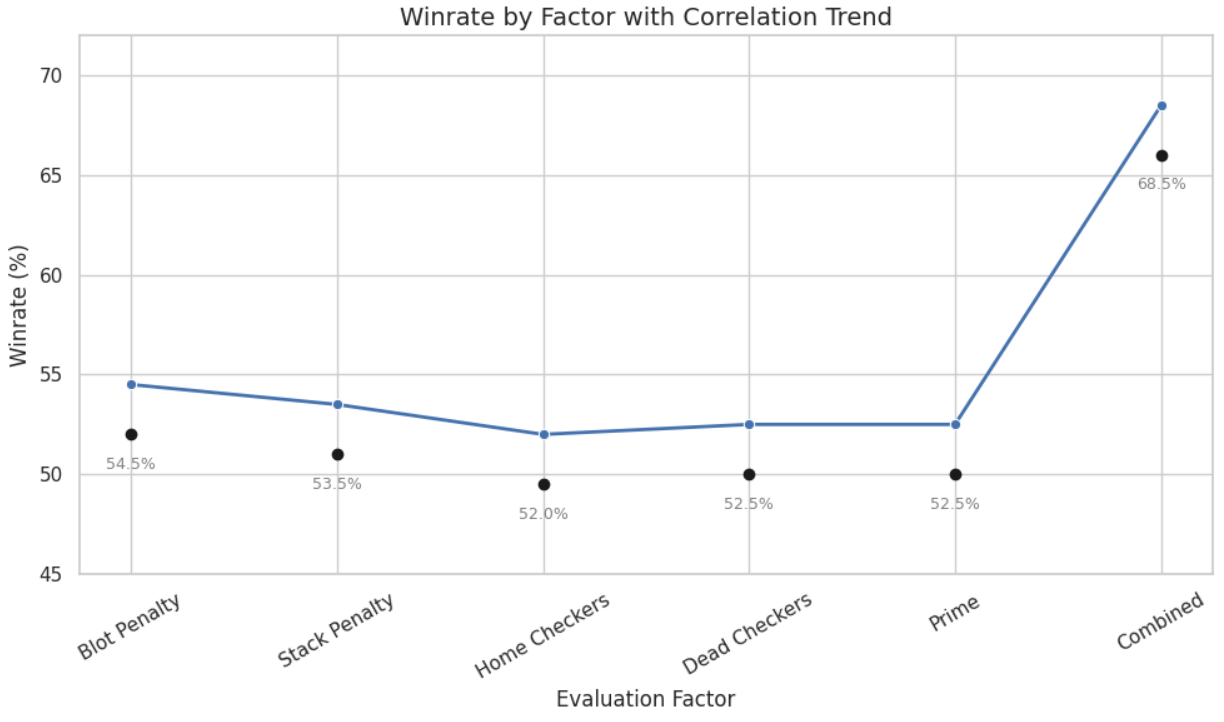
\includegraphics[width=1\linewidth]{obrazky-figures/CorrelationTrend.png}
    \caption{Winrate by Factor}
    \label{Correlation}
\end{figure}

The factors work best together, but even individually, they can make a small improvement. The combination of the home checkers and prime factors proved to be the best. While they did not significantly improve the AI's performance individually, together they created situations where prime was formed close to the player's home zone, which not only blocked the opponent's checkers from leaving the bar, but also blocked the opponent's checkers in the first positions, forcing the opponent to spray his checkers, creating vulnerable zones, or vice versa, to keep too many on one point. This leads to dominance over the opponent, as seen in the figure \ref{fPrime}.

\begin{figure}[H]
    \centering
    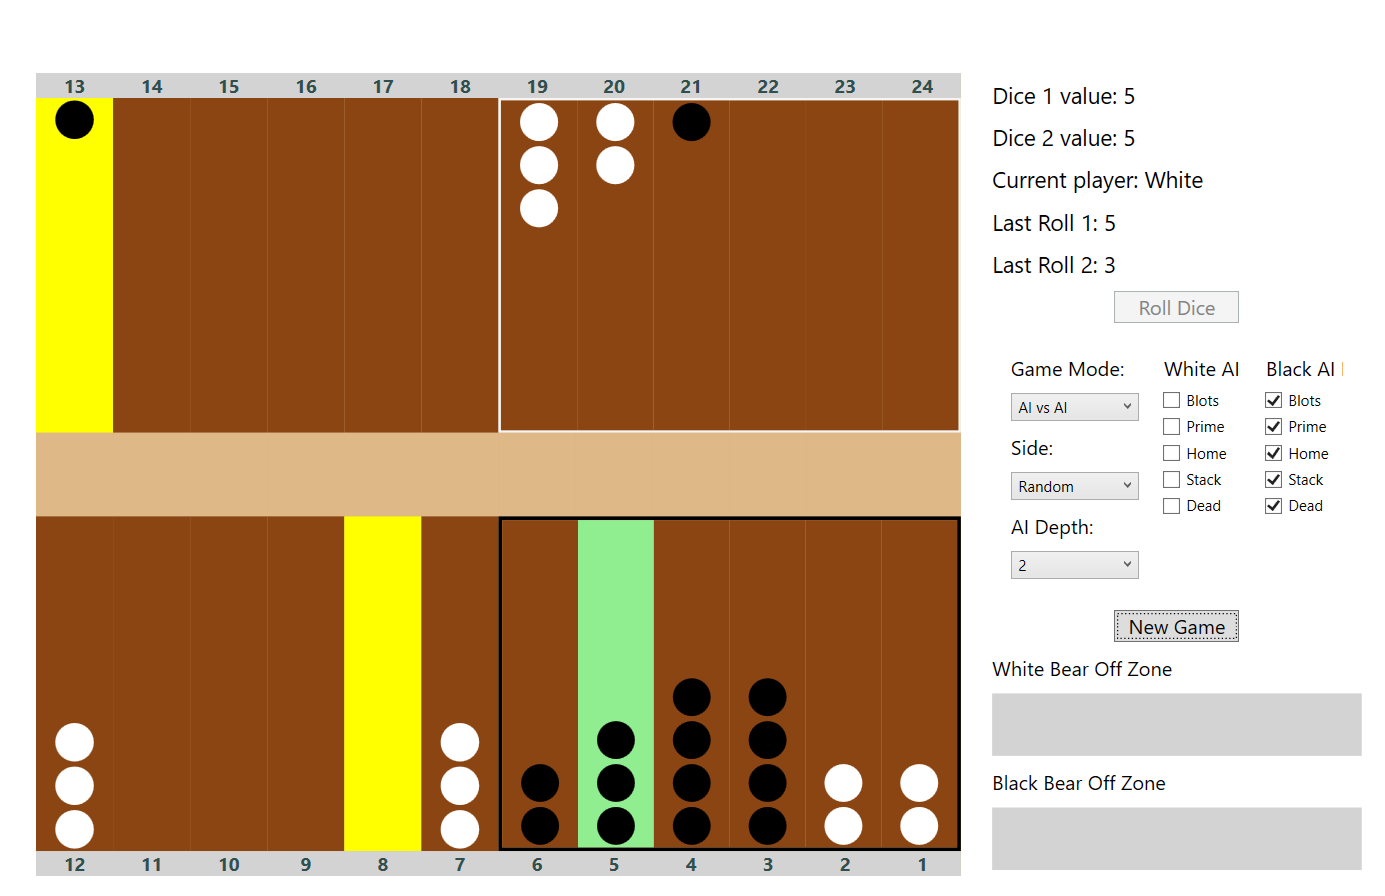
\includegraphics[width=1\linewidth]{obrazky-figures/Prime_example.png}
    \caption{Combination of factors vs base evaluation}
    \label{fPrime}
\end{figure}

Testing individual factors against each other has not yielded any significant results, the winrate of the games played fluctuates around 50\% and it is impossible to judge which factor is stronger than the other. Combinations of factors may be stronger, but they have not been tested enough to claim their superiority with confidence. Nevertheless, the most promising combinations can be identified: Blot Penalty + Stack Penalty, Home Checkers Bonus + Prime Bonus, Home Checkers Bonus + Dead Checkers Penalty.

With all factors enabled, AI becomes fairly strong. If the basic evaluation leads to playing too aggressively, the enabled factors allow it to find very unobvious moves and turn what can be called “luck” in its favor in the long run. Factors play a decisive role in the choice of a move, when the usual score of the basic function ranges up to 100-150, with the factors enabled, which have a cumulative effect, this score is measured in several hundred and often goes over 1000, where the distance in pips no longer plays a major role.
However, these factors have a significant drawback: they do not evaluate the board dynamically. Their impact on the game can be greatly enhanced by adjusting the bonus or penalty modifiers during the game.

\subsection{Tests against human players}

To complement the self-play and statistical experiments, direct human-versus-AI tests were conducted to evaluate how well the AI performs against human intuition and strategic reasoning. Four sets of 15 games were played. Two sets involved a \textbf{beginner} player who had only recently learned the rules of Backgammon. The other two sets were played by a \textbf{seasoned} player with practical experience but no professional training.

Each human opponent played one set against the \textbf{base evaluation} AI (which uses pip count alone) and one set against the \textbf{enhanced evaluation} AI (which includes all implemented factors: blot penalty, stack penalty, home checkers, dead checkers, and prime formation).

The results are summarized in Table~\ref{tab:human_winrate}. The base AI was able to outplay the beginner (9:6), but was significantly outplayed by the seasoned player (5:10), indicating that pip-count-based evaluation alone is not sufficient to withstand even moderate human strategy. However, when all evaluation factors were enabled, the AI showed dramatic improvement. It dominated the beginner player (14:1), and more importantly, reversed its loss against the seasoned player by winning 11 out of 15 games.
\begin{table}[h!]
\centering
\caption{Winrates of AI against human opponents (15 games per set)}
\label{tab:human_winrate}
\begin{tabular}{|l|l|c|}
\hline
\textbf{Opponent Type} & \textbf{AI Configuration} & \textbf{Winrate (AI)} \\
\hline
Beginner& Base Evaluation & 60.0\% (9 / 15)\\
\hline
Beginner& All Factors Enabled & 93.3\% (14 / 15)\\
\hline
Seasoned & Base Evaluation  & 33.3\% (5 / 15)\\
\hline
Seasoned  & All Factors Enabled  & 73.3\% (11 / 15)\\
\hline
\end{tabular}
\end{table}

 Adding factors enabled the AI to recognize and exploit positional weaknesses, avoid tactical errors, and apply consistent pressure—traits.

 Every test in this section had a search depth of 3 plies for the AI player. The average duration of a game varied considerably. The longest games were between the basic evaluation functions, where they simply attacked each other as often as possible and the game sometimes lasted 90 or more moves. The shortest games were between a beginner vs. AI with all factors enabled, and AI with a basic function vs. AI with factors - games lasted about 40 moves where there was complete dominance of AI with factors. On average, the games lasted about 60 moves, which is relatively long.

 The average move time also varied, and it directly depends on the number of available moves and the number of processor cores that calculate the value of the moves. Usually, the calculation time does not exceed 8 seconds, the average value is 5.6 seconds with all factors enabled for a 14-core processor. The basic evaluation function calculates game states about twice as fast as the version with factors. There are cases when there are several hundred possible moves, so the function needs much more time and the calculation can last longer than a minute.  For processors with a small number of cores, the time increases even more.

The use of a transposition table made the algorithm undemanding in terms of RAM usage. Under normal circumstances, the memory usage does not exceed 600-700 MB. For situations where a large number of moves need to be evaluated, this number increased to 2.5~GB, which is not a big amount for modern computers. It allows to run the game even with a search for up to 4 plies. At the same time, the computer's evaluation process takes an extremely long time, several minutes on average for each move, so this use is not advisable.





\chapter{Conclusion}\label{conclusion}
\vspace{-2\baselineskip}
In this work, the goal was to develop a complete implementation of the game of Backgammon, including both the core game logic and a competitive AI. It is based on the ExpectiMiniMax algorithm, which extends the classic MiniMax approach to account for stochastic outcomes, such as dice rolls.

To enhance the decision-making capabilities of the AI, there was created a modular evaluation function. The base layer of the evaluation uses pip count — a standard measure of progress in backgammon — to estimate the desirability of a game state. On top of this, a series of strategically motivated evaluation factors were introduced. This is a set of bonuses and penalties designed to make the position score more “fair”.

Through testing, both in self-play and against human opponents, it was shown that even though individual factors yield modest improvements, their combined effect produces a significantly stronger AI. The enhanced evaluation function outperformed the baseline both statistically and in real-world games. These results confirm that strategic factors, when integrated into a structured evaluation model, can elevate AI performance in complex and probabilistic games like Backgammon.

Various ways to optimize the algorithm have been explored and implemented, and there is still some room for further optimization.

\subsubsection{Final thoughts}
 The algorithm turned out to be strong enough to beat experienced player, but at the same time, I assume that it will not be able to cope against players who have studied the Backgammon game theory well, and most importantly, can dynamically change their tactics. The algorithm itself cannot switch between aggressive and safe play directly. It does not take into account additional factors that also have an impact on the game, but did not statistically show themselves well in this particular case. These are anchors, strategically important points on the board (not all are the same), areas for forming attacks, and so on. Such factors will overload the evaluation function, which is called many times, so I had to choose most relevant. Professional players think about these parts of the strategy as well and manage resources more wisely. 
In fact, the ExpectiMiniMax algorithm is close to its peak at the moment, and further optimizations may create a completely new algorithm from it. The factors found are useful for use in neural networks, for example, which is a more promising approach. Nevertheless, the implemented version is enough to make the game playable and interesting for most people, while the complexity can be adjusted by adding different factors, and it is possible to play with different combinations of them.